\documentclass[a4paper,ngerman,bibtotoc]{scrartcl}

\usepackage[utf8]{inputenc}

\usepackage[ngerman]{babel}

\usepackage{amsmath,amsthm,amssymb,stmaryrd,color,graphicx,extarrows,multirow,subcaption}
\usepackage{bussproofs}
\usepackage{array}
\usepackage{comment}

\usepackage[protrusion=true,expansion=true]{microtype}

\usepackage{lmodern}
\usepackage{tabto}

\usepackage[backend=bibtex,style=alphabetic]{biblatex}
\usepackage[babel]{csquotes}
\bibliography{literatur}

\usepackage[all]{xy}

\usepackage{tikz}
\usetikzlibrary{shapes,arrows}

\usepackage{lscape}				%Querformat
\usepackage{rotating}

\usepackage[colorlinks=true, linkcolor=blue, urlcolor=blue, citecolor=blue]{hyperref}
%\usepackage[colorlinks=true, linkcolor=black, urlcolor=black, citecolor=black]{hyperref}
\usepackage{cleveref}			%Referenzen mit Name


\allowdisplaybreaks


\setlength\parskip{\medskipamount}
\setlength\parindent{0pt}

\theoremstyle{definition}
\newtheorem{defn}{Definition}[section]
\newtheorem{bsp}[defn]{Beispiel}

\theoremstyle{plain}
\newtheorem{prop}[defn]{Proposition}
\crefname{prop}{Proposition}{Prop.}
\newtheorem{lemma}[defn]{Lemma}
\newtheorem{kor}[defn]{Korollar}
\newtheorem{satz}[defn]{Satz}

\theoremstyle{remark}
\newtheorem{bem}[defn]{Bemerkung}

\newcommand{\CC}{\mathbb{C}}
\newcommand{\NN}{\mathbb{N}}
\newcommand{\RR}{\mathbb{R}}
\renewcommand{\exp}[1]{\textup{exp}\left(#1\right)}
\newcommand{\A}{A}
\newcommand{\B}{B}
\newcommand{\C}{C}
\newcommand{\D}{D}
\newcommand{\KatC}{\mathbf{C}}
\newcommand{\KatD}{\mathbf{D}}
\newcommand{\stetig}{\mathfrak{C}}
\newcommand{\SpecC}{\mathfrak{Spec}}
\newcommand{\kommentar}{\color[rgb]{1,0,0}}


\newcommand{\TopMan}{\mathrm{TopMan_c}}
\newcommand{\CMan}{\mathrm{C\text{*}Man}}
\newcommand{\tpsii}{\widetilde{\psi_i}}
\newcommand{\hpsii}{\widehat{\psi_i}}


\newcommand{\CAlg}{C*-Algebra}
\newcommand{\CAlgn}{C*-Algebren}
\newcommand{\CAlgMan}{C*-Algebra-Mannigfaltigkeit}
\newcommand{\CAlgMann}{C*-Algebra-Mannigfaltigkeiten}
\newcommand{\komTopMan}{kompakte topologische Mannigfaltigkeit}
\newcommand{\komTopMann}{kompakte topologische Mannigfaltigkeiten}
\newcommand{\komenTopMan}{kompakten topologischen Mannigfaltigkeit}
\newcommand{\CAlgHom}{$*$-Homomorphismus}
\newcommand{\CAlgHomn}{$*$-Homomorphismen}
\newcommand{\ssTop}{schwach-$*$-Topologie}
\newcommand{\Beh}{\underline{Behauptung:} }
\newcommand{\Ann}{\underline{Annahme:} }
\newcommand{\Fall}[1]{\underline{#1. Fall:} }
\newcommand{\Bew}[1]{Beweis (Satz v. GN - #1)}

\newcommand{\eval}{\varepsilon}						%Evaluationsabbildung
\newcommand{\lima}{L(a)}							%lim ||a^k||^(1/k)
\newcommand{\AlgIso}{H}								%Der Isomorphismus im Satz von Gelfand-Neumark
\newcommand{\Homoeo}{\Phi}							%Standardhomöomorphismus
\newcommand{\dual}[1]{\widetilde{#1}}				%Der Dualraum des Raumes "1"
\newcommand{\norm}[1]{\left\lVert#1\right\rVert}	% ||#1|| (passt sich der Größe an)

\newcommand{\Hom}{\mathrm{Hom}}
\newcommand{\id}{id}
\newcommand{\Id}{\mathfrak{Id}}
\newcommand{\Funk}{\mathfrak{F}}
\newcommand{\Gunk}{\mathfrak{G}}

\newcommand{\KatCAlg}{\mathbf{C^*Alg}}
\newcommand{\KatCAlgMan}{\mathbf{C^*AlgMan}}
\newcommand{\KatTop}{\mathbf{Top}}
\newcommand{\KatTopMan}{\mathbf{TopMan}}
\newcommand{\op}{\mathrm{op}}

%Eine eigene Liste für Listen in Propositionen, deren Punkte direkt referenziert werden sollen ( http://tex.stackexchange.com/questions/156049/how-can-i-get-cleveref-enumitem-to-print-not-item-e-but-proposition-1 )
\usepackage{enumitem}
\newlist{propenum}{enumerate}{1} 					% also creates a counter called 'propenumi'
%label=... definiert die Form der Numerierung, ref=... die Form der Referenzierung (theprop für Umgebung prop)
\setlist[propenum]{label=\textup{\alph*)}, ref=\theprop~(\alph*)}
\crefalias{propenumi}{prop} 

%Analog für Beweise:
\newlist{proofenum}{enumerate}{1} 					
\setlist[proofenum]{label=\textup{\alph*)}, ref=\alph*)}
\crefalias{proofenumi}{proof}

%und für Definitionen:
\newlist{defenum}{enumerate}{1} 					
\setlist[defenum]{label=\textup{\arabic*.}, ref=Eigenschaft~\arabic*}
\crefalias{defenumi}{defn}

\newcounter{temp}									% Eigener Counter für Fortsetzung von Zählungen 



\clubpenalty=10000
\widowpenalty=10000
\displaywidowpenalty=10000

\newenvironment{indentblock}{%
  \list{}{\leftmargin\leftmargin}%
  \item\relax
}{%
  \endlist
}


\title{Bachelorarbeit}
\author{Lukas Graf}



\begin{document}

\begin{titlepage}\center
\textsc{\LARGE Universität Augsburg}\\[1.5cm]

\textsc{\Large Institut für Mathematik}\\[2.5cm]

% Title
{ \huge \bfseries Bachelorarbeit \\[1.5cm]
\Large Der Satz von Gelfand-Neumark und eine Erweiterung für topologische Mannigfaltigkeiten \\[6cm] }



\vfill

% Author and supervisor
\begin{minipage}{0.4\textwidth}
\begin{flushleft} \large
\emph{Vorgelegt von:}\\
 Lukas \textsc{Graf}
\end{flushleft}
\end{minipage}
\begin{minipage}{0.4\textwidth}
\begin{flushright} \large
\emph{Betreut von:} \\
 Prof. Dr. Kai \textsc{Cieliebak}
\end{flushright}
\end{minipage}

\end{titlepage}


\tableofcontents

\newpage

\phantomsection
\addcontentsline{toc}{section}{Einleitung}
\section*{Einleitung}

\begin{center}
Was haben die komplexen Zahlen und ein Raum aus einem einzigen Punkt gemeinsam? 
\end{center}

Eine etwas seltsame Frage vielleicht - nichtsdestotrotz wird die folgende Arbeit eine Antwort darauf liefern. Genauer gesagt handelt es sich dabei um den einfachsten Spezialfall des Satzes von Gelfand-Neumark. Dieser stellt nämlich eine solche Verbindung zwischen \CAlgn{} (einer Art Verallgemeinerung der komplexen Zahlen) auf der einen Seite und gewissen topologischen Räumen auf der anderen Seite her. 

Die Aussage des Satzes von Gelfand-Neumark ist, in der hier betrachteten Fassung\footnote{In seiner ursprünglichen 1943 von Israel Gelfand und Mark Neumark bewiesenen Variante (\cite[Theorem 1]{GN1943}) gilt der Satz auch für nicht-kommutative \CAlgn{} (dort als \glqq normed $*$-ring\grqq{} bezeichnet). Wir werden uns im Folgenden aber auf kommutative \CAlgn{} beschränken, was im originalen Artikel dem ersten Lemma entspricht.}, dass jede \CAlg{} auch als der Raum der stetigen, komplexwertigen Funktionen über einem bestimmten kompakten Hausdorffraum gesehen werden kann (bis auf eine längentreue Isomorphie). Das erste Kapitel der folgenden Arbeit widmet sich - einem Vorlesungsskript von Christian Bär (\cite[S. 49-69]{Baer2003}) folgend - der Definition der notwendigen Begriffe und dem Beweis dieses Satzes.

Daran anschließend werden wir der \glqq umgedrehten\grqq{} Fragestellung nachgehen - d.h. untersuchen, ob auch jeder kompakter Hausdorffraum als Funktionenraum über einer \CAlg{} betrachtet werden kann. Tatsächlich ist dies der Fall und führt zur Gelfand-Dualität, um die es im zweiten Kapitel gehen wird. Diese besagt, dass \CAlgn{} und kompakte Hausdorffräume in einem gewissen Sinne äquivalent zueinander sind - oder, genauer gesagt, dual zueinander.

Im dritten Kapitel schließlich werden wir eine besondere Art von kompakten Hausdorffräumen herausgreifen - die topologischen Mannigfaltigkeiten - und versuchen, die Aussagen der Sätze der vorangegangen Kapitel dafür zu erweitern. Insbesondere werden wir uns dabei fragen:

\begin{center}
Wie kann man einer \CAlg{} \glqq ansehen\grqq{}, ob der zu ihr duale kompakte Hausdorffraum eine topologischen Mannigfaltigkeit ist?
\end{center}
\newpage
\section{Der Satz von Gelfand-Neumark}\label{sec:GN}

\subsection{Definitionen}

In diesem Kapitel werden die zur Formulierung des Satzes von Gelfand-Neumark notwendigen Objekte definiert. Außerdem werden wir zu diesen einige grundlegende Eigenschaften zeigen, die für den späteren Beweis hilfreich sein werden.

\begin{defn}[Banachalgebra]
Eine \emph{kommutative komplexe Banachalgebra mit Eins} ist ein $\CC$-Vektorraum, mit einer kommutativen Multiplikation, einem Einselement und einer submultiplikativen Norm, bezüglich der er vollständig ist.

D.h. eine kommutative komplexe Banachalgebra mit Eins ist ein $\CC$-Vektorraum $(\A, +)$ mit einer Operationen $\cdot: \A \times \A \to \A: (a,b) \mapsto a\cdot b$, sodass
\begin{itemize}
	\item $\forall a,b,c  \in \A: a\cdot(b+c) = a\cdot b + a\cdot c$ (Distributivität)
	\item $\forall a,b \in A, \lambda \in \CC: \lambda(a\cdot b) = (\lambda a)\cdot b$
	\item $\forall a,b,c \in \A: (a\cdot b)\cdot c = a \cdot (b \cdot c)$ (Assoziativität)
	\item $\forall a, b \in \A: a\cdot b = b \cdot a$ (Kommutativität),	
\end{itemize}
einem ausgezeichneten Element $e \in \A \backslash \{0\}$, sodass
\begin{itemize}
	\item $\forall a \in \A: e\cdot a = a$ (Einselement),
\end{itemize}
sowie einer Normabbildung $\norm{.}: \A \to \RR_{\geq0}: a \mapsto \norm{a}$, sodass
\begin{itemize}
	\item $\forall a,b \in \A: \norm{a \cdot b} \leq \norm{a} \cdot \norm{b}$ (Submultiplikativität)
\end{itemize}
und $(\A, \norm{.})$ vollständig ist.

Die \emph{Dimension} einer Banachalgebra ist die Dimension des ihr zugrunde liegenden Vektorraums.
\end{defn}

\begin{bem}
Da im Folgenden ausschließlich kommutative und komplexe Banachalgebren mit Eins betrachtet werden, nennen wir diese ab sofort kurz \emph{Banachalgebren}. Wie für Multiplikationen üblich wird außerdem oft $ab$ statt $a \cdot b$ verwendet werden.
\end{bem}

\begin{bem}
Gibt es zu einem $a \in \A$ ein $b \in \A$ mit $ab = e$, so ist dieses $b$ eindeutig. Denn gäbe es ein $c \in \A$ mit der gleichen Eigenschaft, so wäre:
	\[c = ce = c(ab) = (ac)b = eb = b\]
Wir nennen ein solches $b$ \emph{Inverses} zu $a$ und bezeichnen es mit $a^{-1}$. Die Menge aller invertierbaren Elemente von $\A$ bezeichnen wir mit $\A^\times$.
\end{bem}

\begin{lemma}\label{lemma:BAlg-Eigenschaften}
Ist $\A$ eine Banachalgebra, so sind folgende Abbildungen stetig:
\begin{itemize}
	\item $\A \times \A \to \A: (a,b) \mapsto a+b$
	\item $\A \times \A \to \A: (a,b) \mapsto a\cdot b$	
	\item $\CC \times \A \to \A: (\lambda,a) \mapsto \lambda a$
	\item $\A^\times \to \A^\times: a \mapsto a^{-1}$
\end{itemize}
\end{lemma}

\begin{proof}Wir folgen hier dem Beweis zu \cite[Lemma 2.1.14]{Baer2003}.

Seien $a_0, b_0 \in \A, \lambda_0 \in \CC$ und $\epsilon > 0$. Dann gilt:
\begin{itemize}
\item Für alle $a,b \in \A$ mit $\norm{a-a_0}$, $\norm{b-b_0} < \frac{\epsilon}{2}$ ist
		\[\norm{(a+b) - (a_0+b_0)} \leq \norm{a-a_0} + \norm{b-b_0} < \frac{\epsilon}{2} + \frac{\epsilon}{2} = \epsilon.\]
		Also ist die Addition stetig.
		
\item Für alle $a,b \in \A$ mit $\norm{a-a_0}$, $\norm{b-b_0} < \min\left\lbrace\sqrt{\frac{\epsilon}{3}}, \frac{\epsilon}{3\norm{a_0}}, \frac{\epsilon}{3\norm{b_0}}\right\rbrace$ ist
		\begin{align*}
		\norm{ab - a_0b_0} = \norm{ab -a_0b +a_0b -a_0b_0} = \norm{(a-a_0)b + (b-b_0)a_0} \leq \\
		\leq \norm{a-a_0}\norm{b} + \norm{b-b_0}\norm{a} = \norm{a-a_0}\norm{b-b_0+b_0} + \norm{b-b_0}\norm{a_0} \leq \\
		\leq \norm{a-a_0}\norm{b-b_0} + \norm{a-a_0}\norm{b_0} + \norm{b-b_0}\norm{a_0} < \\
		< \sqrt{\frac{\epsilon}{3}} \sqrt{\frac{\epsilon}{3}} + \frac{\epsilon}{3\norm{b_0}}\norm{b_0} + \frac{\epsilon}{3\norm{a_0}}\norm{a_0} = \frac{\epsilon}{3} + \frac{\epsilon}{3} + \frac{\epsilon}{3} = \epsilon.		
		\end{align*}
		Also ist die Multiplikation stetig.
		
\item Für alle $\lambda \in \CC$ mit $|\lambda - \lambda_0| < \frac{\epsilon}{\norm{e}}$ ist
		\[\norm{\lambda e - \lambda_0 e} = \norm{(\lambda-\lambda_0)e} = |\lambda - \lambda_0| \norm{e} < \epsilon.\]
		Also ist die Skalarmultiplikation $(\lambda,a) \mapsto \lambda a$ als Verknüpfung der stetigen Abbildungen $(\lambda,a) \mapsto (\lambda e,a)$ und $(\lambda e, a) \mapsto \lambda e \cdot a = \lambda a$ ebenfalls stetig.
		
\item Ist $a_0 \in \A^\times$, so ist für alle $a \in \A^\times$ mit $\norm{a-a_0}~<~\frac{\epsilon}{\norm{a_0^{-1}}^2+\norm{a_0^{-1}}\epsilon}$:
	\begin{align*}
	\norm{a^{-1}-a_0^{-1}} = \norm{a^{-1}a_0a_0^{-1}-a^{-1}aa_0^{-1}} = \norm{a^{-1}(a_0-a)a_0^{-1}} \leq \\
	\norm{a^{-1}}\norm{a-a_0}\norm{a_0^{-1}} = \norm{a^{-1}-a_0^{-1}+a_0^{-1}}\norm{a-a_0}\norm{a_0^{-1}} \leq \\
	\norm{a^{-1}-a_0^{-1}}\norm{a-a_0}\norm{a_0^{-1}} + \norm{a_0^{-1}}\norm{a-a_0}\norm{a_0^{-1}}
	\end{align*}
Also
	\[\norm{a^{-1}-a_0^{-1}}\left(1 - \norm{a-a_0}\norm{a_0^{-1}}\right) \leq \norm{a-a_0}\norm{a_0^{-1}}^2\]
und wegen
	\[1-\norm{a-a_0}\norm{a_0^{-1}} > 1 - \frac{\epsilon}{\norm{a_0^{-1}}^2+\norm{a_0^{-1}}\epsilon} \norm{a_0^{-1}} = \frac{\norm{a_0^{-1}} + \epsilon - \epsilon}{\norm{a_0^{-1}}+\epsilon} > 0\]
folgt
	\[\norm{a^{-1}-a_0^{-1}} \leq \frac{\norm{a-a_0}\norm{a_0^{-1}}^2}{1 - \norm{a-a_0}\norm{a_0^{-1}}}.\]
Außerdem gilt:
	\begin{align*}
	\norm{a-a_0} < \frac{\epsilon}{\norm{a_0^{-1}}^2+\norm{a_0^{-1}}\epsilon} 
	\Rightarrow \norm{a-a_0}\left(\norm{a_0^{-1}}^2+\norm{a_0^{-1}}\epsilon\right) < \epsilon \\ 
	\Rightarrow \norm{a-a_0}\norm{a_0^{-1}}^2 < \epsilon\left(1-\norm{a-a_0}\norm{a_0^{-1}}\right) 
	\Rightarrow \frac{\norm{a-a_0}\norm{a_0^{-1}}^2}{1-\norm{a-a_0}\norm{a_0^{-1}}} < \epsilon
	\end{align*}
Also ist $\norm{a^{-1}-a_0^{-1}}< \epsilon$ und somit die Inversenbildung stetig.

\end{itemize}
\end{proof}

\begin{defn}[C*-Algebra]
Eine \emph{kommutative \CAlg{} mit Eins} ist eine Banachalgebra $(\A, +, \cdot, e, \norm{.})$ zusammen mit einer Involutionsabbildung $(~)^*:\A \to \A$, die verträglich ist mit der Algebra-Struktur und der Norm.

D.h. für die Involutionsabbildung soll gelten:
\begin{itemize}
	\item $\forall a  \in \A: (a^*)^* = a$ (Involutionseigenschaft)
	\item $\forall a,b \in \A, \lambda \in \CC: (\lambda a + b)^* = \overline{\lambda}a^* + b^*$ (verträglich mit der  Vektorraumstruktur)
	\item $\forall a,b \in \A: (a\cdot b)^* = b^*\cdot a^*$ (verträglich mit der Multiplikation)
	\item $\forall a \in \A: \norm{a^*\cdot a} = \norm{a}^2$ (verträglich mit der Norm)
\end{itemize}
\end{defn}

\begin{bem}
Auch die kommutativen \CAlgn{} mit Eins werden wir ab sofort kurz als \emph{\CAlgn} bezeichnen.
\end{bem}

\begin{kor}\label{lemma:CAlg-Eigenschaften}
Ist $\A$ eine \CAlg{}, so gilt $e^* = e$ und $\norm{e} = 1$
\end{kor}

\begin{proof}%Entspricht Bem2.1.4
Für das Einselement $e$ einer \CAlg{} ist
	\[e^* = ee^* = (ee^*)^{**} = (e^{**}e^*)^* = (ee^*)^* = (e^*)^* = e\]
und
	\[\norm{e}^2 = \norm{e^*e} = \norm{ee} = \norm{e}.\]
Also muss $\norm{e} = 1$ gelten ($\norm{e} \neq 0$, da $e \neq 0$).
\end{proof}


\begin{defn}[\CAlgHom/Isometrie]\label{defn:AlgHom}\label{defn:CAlgHom}\label{defn:CAlgIso}\label{defn:Isometrie}
Seien $\A, \B$ zwei \CAlgn, dann heißt eine Abbildung $h: \A \to \B$ 
\begin{enumerate}
\item\emph{Algebrenhomomorphismus}, wenn gilt
\begin{itemize}
	\item $\forall a,b \in \A, \lambda \in \CC: h(\lambda a + b) = \lambda h(a) + h(b)$ (linear)
	\item $\forall a,b \in \A: h(ab) = h(a)h(b)$ (multiplikativ)
	\item $h(e) = e$ (einserhaltend)
\end{itemize}

\item\emph{{\CAlgHom}}, wenn zusätzlich gilt:
\begin{itemize}
	\item $\forall a \in \A: h(a^*) = \big(h(a)\big)^*$
\end{itemize}

\item\emph{Isomorphismus von \CAlgn}, wenn $h$ außerdem biijektiv ist.

\item\emph{Isometrie} bzw. \emph{isometrisch}, wenn gilt:
\begin{itemize}
	\item $\forall a \in \A: \norm{h(a)} = \norm{a}$
\end{itemize}

\end{enumerate}
\end{defn}

\begin{bem}
Ein \CAlgHom{} ist immer auch stetig (bzgl. der von den Normen der \CAlgn{} induzierten Topologien), ein Isomorphismus von \CAlgn{} ist sogar immer isometrisch. Ein Beweis hierfür findet sich in  \cite[Korollare 2.1.19 \& 2.1.20]{Baer2003}.
\end{bem}


\begin{defn}[kompakter Hausdorffraum]
Ein \emph{kompakter Hausdorffraum} ist eine Menge $X$ zusammen mit einer Topologie auf $X$, sodass gilt:
\begin{itemize}
	\item Sind $U_i \subseteq X, i \in I$ offene Mengen mit $\bigcup_{i\in I} U_i = X$ (dann heißt $(U_i)_{i \in I}$ \emph{Überdeckung} von $X$), so gibt es eine endliche Teilmenge $J \subseteq I$ mit $\bigcup_{i\in J} U_i = X$ (Kompaktheit).
	\item Sind $x \neq y \in X$ zwei verschiedene Punkte in $X$, so gibt es offene Mengen $U,V \subset X$ mit $x \in U, y \in V$ und $U \cap V = \emptyset$ (Hausdorffeigenschaft).
\end{itemize}
\end{defn}

\begin{defn}[Homöomorphismus]
Seien $X, Y$ zwei topologische Räume. Dann heißt eine Abbildung $\varphi: X \to Y$ \emph{Homöomorphismus}, wenn sie bijektiv ist und sowohl $\varphi$ als auch $\varphi^{-1}$ stetig sind.
\end{defn}

\begin{lemma}\label{lemma:komHDHomoeo}
Ist $X$ ein kompakter topologischer Raum, $Y$ ein Hausdorffraum und $\varphi: X \to Y$ eine stetige bijektive Abbildung, so ist auch $\varphi^{-1}$ stetig (und damit $\varphi$ ein Homöomorphismus).
\end{lemma}

\begin{proof}Sei $U \subseteq X$ offen. Zu zeigen ist, dass dann auch $\varphi(U) \subseteq Y$ offen ist, d.h. jedes $y_0 \in \varphi(U)$ eine offene Umgebung in $\varphi(U)$ hat.

Da $Y$ hausdorffsch ist, gibt es zu jedem $y \in Y \backslash \varphi(U)$ offene disjunkte Mengen $V_y, W_y \subset Y$ mit $y_0 \in V_y$ und $y \in W_y$. Dann ist $(\varphi^{-1}(W_y))_{y \in Y\backslash \varphi(U)}$ eine offene Überdeckung von $X \backslash U$, denn:
\begin{itemize}
	\item Die $W_y$ sind offen und $\varphi$ ist stetig. Also sind auch die $\varphi^{-1}(W_y)$ offen.
	\item Ist $x \in X \backslash U$, so ist, da $\varphi$ bijektiv ist, $y := \varphi(x) \in Y \backslash \varphi(U)$. Daher ist $x \in \varphi^{-1}(W_y)$ für ein $y \in Y \backslash \varphi(U)$. 
\end{itemize}

$X \backslash U$ ist als abgeschlossene Teilmenge einer kompakten Menge selbst kompakt. Folglich gibt es eine endliche Menge $M \subseteq Y \backslash \varphi(U)$, sodass $X \backslash U \subseteq \bigcup_{y \in M}\varphi^{-1}(W_y)$ ist. Also ist $\bigcap_{y \in M}\varphi^{-1}(V_y) \subseteq U$ und daher $\bigcap_{y \in M}V_y \subseteq \varphi(U)$ eine offene Umgebung von $y_0$.
\end{proof}

\subsection{$\CC^n$ als Beispiel einer \CAlg}\label{sec:BeispielCn}

Bevor wir zum eigentlichen Satz von Gelfand-Neumark kommen, werden wir ihn in diesem Abschnitt zunächst am Spezialfall des $\CC^n$ betrachten. Dieser wird mit komponentenweiser Multiplikation, der Maximumsnorm $||.||_\infty$ und der Involutionsabbildung
\[*: 
\left(\begin{matrix}
 c_1 \\ \vdots \\ c_n 
\end{matrix}\right)
\mapsto 
\left(\begin{matrix}
\overline{c_1} \\ \vdots \\ \overline{c_n}
\end{matrix}\right) \qquad (\overline{c_k} \text{ sei die komplexe Konjugation von } c_k  \text{ in } \CC).\]
eine ($n$-dimensionale) \CAlg{}. Die Einheitsvektoren $e_k = \left( \delta_{1k} \  \dots \ \delta_{nk} \right)^T$ bilden dann eine Basis dieser \CAlg{} und $e := (1,\dots,1)^T = \sum_{k=1}^ne_k$ ist ihr Einselement.

Als erstes wollen wir einen kompakten Hausdorffraum zu dieser \CAlg{} konstruieren. Betrachten wir dazu die Menge
	\[\SpecC(\CC^n) := \{f: \CC^n \to \CC ~|~ f \text{ stetiger Algebrenhomomorphismus}\},\]
so gilt für jeden Algebrenhomomorphismus $f \in \SpecC(\CC^n)$:
	\[f(e_k) = f(e_k \cdot e_k) \overset{Alg.hom.}{=} f(e_k) \cdot f(e_k) \in \CC\]
Also $f(e_k) \in \{0, 1\}$. Gleichzeitig gilt aber auch:
	\[1 = f(e) = f\left(\sum_{k=1}^n e_k\right) \overset{Alg.hom.}{=} \sum_{k=1}^n f(e_k)\]
Insgesamt gibt es daher genau ein $k_f \in \{1, \dots, n\}$ mit $f(e_{k_f}) = 1$. Und durch dieses ist $f$ bereits eindeutig festgelegt, denn es gilt:
	\[\forall c \in \CC^n: f(c) = f\left(\sum_{k=1}^n c_k e_k\right) \overset{Alg.hom.}{=} \sum_{k=1}^n c_k f(e_k) = c_{k_f} \]
Einfaches Nachrechnen zeigt, dass die so definierten $n$ verschiedenen Abbildungen tatsächlich stetige Algebrenhomomorphismen sind. Also ist $\SpecC(\CC^n)$ eine Menge aus $n$ Elementen $\{f_1, \dots, f_n\}$. Versehen mit der diskreten Topologie (jede Teilmenge ist eine offene Menge) wird $\SpecC(\CC^n)$ so offensichtlich zu einem kompakter Hausdorffraum.

Betrachten wir auf diesem Raum nun die Menge der stetigen Abbildungen nach $\CC$:
	\[\stetig(\SpecC(\CC^n)) := \{\tau: \SpecC(\CC^n) \to \CC ~|~ \tau \text{ stetig}\}\]
Versehen wir diese auf natürliche Weise mit der Struktur einer Algebra, der Maximumsnorm $\norm{\tau} := \max \{|\tau(f)| ~|~ f \in \SpecC(\CC^n)\}$ und der komplexen Konjugation als Involution, so wird $\stetig(\SpecC(\CC^n))$ eine \CAlg. 

Da $\SpecC(\CC^n)$ aus genau $n$ verschiedenen Elementen besteht, ist eine Funktion $\tau$ auf diesem Raum definiert durch die Werte von $\tau$ auf diesen $n$ Punkten von $\SpecC(\CC^n)$. Außerdem ist aufgrund der diskreten Topologie \emph{jede} Funktion auf $\SpecC(\CC^n)$ auch stetig. Damit ist die folgende Abbildung bijektiv:
	\[\AlgIso: \CC^n  \to \stetig(\SpecC(\CC^n)): \left(\begin{matrix} c_1 \\ \vdots \\ c_n \end{matrix}\right) \mapsto (\tau_c: \SpecC(\CC^n) \to \CC: f_k \mapsto c_k) \]
Es ist jetzt leicht zu zeigen, dass $\AlgIso$ ein isometrischer Isomorphismus ist.

Insgesamt haben wir also einen kompakten Hausdorffraum gefunden (nämlich $\SpecC(\CC^n)$), dessen Funktionenraum isometrisch isomorph zu unserer ursprünglichen \CAlg{} $\CC^n$ ist.

Eine vergleichbare Konstruktion wollen wir im Folgenden auch für allgemeine \CAlgn{} finden. Dazu werden wir als erstes die Konstruktionen von $\SpecC(\CC^n)$ und $\stetig(\SpecC(\CC^n))$ verallgemeinern:

\subsection{$\SpecC(\A)$ als kompakter Hausdorffraum}\label{sec:SpecCA}

Analog zum obigen Beispiel soll auch für eine beliebige \CAlg{} $\A$ die Menge der stetigen Algebrenhomomorphismen von $\A$ nach $\CC$ als zugehörigen topologischen Raum verwendet werden. Da dieser im Allgemeinen nicht endlich sein muss, wäre die diskrete Topologie hierfür jedoch zu fein und der Raum damit nicht mehr kompakt. Stattdessen werden wir die folgende Topologie verwenden:

\begin{defn}[\ssTop]\label{defn:schwachSternTop}
Sei $(A, ||.||)$ ein $\CC$-Vektorraum und $\dual{A} := \{f: A \to \CC ~|~ f \text{ stetig, linear}\}$ der zugehörige Dualraum. Die von der Subbasis
\[ U(f_0, a, \epsilon) := \{f \in \A ~|~ |f_0(a)-f(a)| < \epsilon\} ~,~ f_0 \in \dual{\A}, a \in \A, \epsilon > 0\]
erzeugte Topologie auf $\A$ heißt dann \emph{\ssTop}.
\end{defn}

\begin{kor}\label{bem:Einsetz-stetig}
Die \ssTop{} ist gerade so definiert, dass die \emph{Einsetzungsabbildungen} $\eval_a: \dual{\A} \to \CC: f \mapsto f(a)$ für alle $a\in \A$ stetig sind.
\end{kor}

\begin{proof}
Zu $f_0 \in \dual{\A}$, $\epsilon > 0$ betrachte die offene Menge $U(f_0, a, \epsilon) \subseteq \dual{\A}$.
\end{proof}

\begin{bem}
Da $\SpecC(\CC^n)$ aus \cref{sec:BeispielCn} eine Teilmenge von $\dual{\CC^n}$ ist, können wir auch diesen Raum mit der \ssTop{} versehen. Es ist leicht zu sehen, dass sie in diesem Spezialfall der diskreten Topologie entspricht (betrachte die Umgebungen $U(f_k, e_k, {}^1/_2)$.
\end{bem}

\begin{lemma}\label{lemma:MA}
Sei $\A$ eine \CAlg. Dann ist
\[\SpecC(\A) := \{f: \A \to \CC ~|~ f \text{ stetiger Algebrenhomomorphismus}\} \subset \dual{\A}\]
mit der \ssTop{} ein kompakter Hausdorffraum.
\end{lemma}

\begin{proof}
Die Hausdorffeigenschaft für $\SpecC(\A)$ folgt bereits direkt aus der Definition der \ssTop{} (vgl. \cite[Lemma 2.1.27 b)]{Baer2003}): Sind nämlich $f, g \in \SpecC(\A)$ mit $f \neq g$, d.h. $\exists a\in A: f(a) \neq g(a)$, so setzen wir $\epsilon := \frac{1}{2} |f(a) - g(a)| > 0$. Dann sind $U(f, a, \epsilon), U(g, a, \epsilon)$ disjunkte offene Umgebungen von $f$ bzw. $g$. Also ist $\SpecC(\A)$ hausdorffsch.

Für den Beweis der Kompaktheit benötigen wir dagegen einige Hilfsaussagen:

\begin{figure}[h]
	\input{Diagramm-Header}
  
\begin{footnotesize}

\begin{tikzpicture}[node distance = 2cm, auto]
    % Place nodes
	\node [Text] (satz) {$\SpecC(\A)$ ist kompakt};
	\node [below of=satz, node distance=1cm] (hilf-satz) {};
    
    \node [Text, left of=hilf-satz] (Spec0-komp) {$\SpecC(\A)\cup\{0\}$ komp.};    
    \node [keinBeweis, below of=Spec0-komp, text width=10em, node distance=1.5cm] (B0-komp) 
    	{\Cref{satz:BA} \\ $\dual{B_1}(0) \subseteq \dual\A$ komp.}; 
    \node [Prop, left of=B0-komp, text width=10em, node distance=4cm] (Spec-in-B0) {\Cref{prop:Spec-in-B0} \\ $\SpecC(\A)\cup\{0\} \subseteq \dual{B_1}(0)$};
    \node [Prop, right of=B0-komp, text width=10em, node distance=4cm] (Spec0-abg) {\Cref{prop:Spec0-abg} \\ $\SpecC(\A) \cup \{0\} \subseteq \dual{\A}$ abg.};
         
	\node [Prop, right of=hilf-satz, text width=13em, node distance=5cm] (Spec-abg) {\Cref{prop:Spec-abg} \\ $\SpecC(\A) \subseteq \SpecC(\A)\cup\{0\}$ abg.};   
	
	\node [Text, below of=Spec0-abg, text width=13em, node distance=1.5cm] (Einsetz-stetig) {\Cref{bem:Einsetz-stetig} \\ $\eval_a: \dual{A} \to \CC: f \mapsto f(a)$ stetig};
                                
    % Draw edges
	\path [line] (Spec0-komp) -- (satz);
	\path [line] (B0-komp) -- (Spec0-komp);
	\path [line] (Spec-in-B0) -- (Spec0-komp);
	\path [line] (Spec0-abg) -- (Spec0-komp);
	
	\path [line] (Spec-abg) -- (satz);	
	
	\path [line] (Einsetz-stetig) -| (Spec-abg);      
	\path [line] (Einsetz-stetig) -- (Spec0-abg);      
		
\end{tikzpicture}



\end{footnotesize}
	\caption{Der Aufbau des Beweises zu \cref*{lemma:MA}}
\end{figure}


\begin{prop}
Sei $\A$ eine \CAlg{} und $\dual{\A}$ der Dualraum dazu, versehen mit der schwach-*-Topologie. Sei $0$ die Nullabbildung in $\dual{\A}$ und $\dual{B_1}(0) \subseteq \dual{\A}$ die abgeschlossene Einheitskugel bezüglich der induzierten Norm. Dann gilt:
\begin{propenum}
	\item $\SpecC(\A) \cup \{0\} \subseteq \dual{\A}$ ist abgeschlossen. 		\label{prop:Spec0-abg} 
	\item $\SpecC(\A) \subseteq \SpecC(\A) \cup \{0\}$ ist abgeschlossen.		\label{prop:Spec-abg} 
	\item $\SpecC(\A) \subseteq \dual{B_1}(0)$							\label{prop:Spec-in-B0} 
\end{propenum}
\end{prop}

\begin{proof}Der Beweis zu \ref*{prop:Spec0-abg} und \ref*{prop:Spec-abg} folgt dem zu \cite[Lemma 2.1.27 a), d)]{Baer2003}.
\begin{proofenum} 
	\item %Folgt 2.1.27a
	Für beliebige $a, b \in \A$ definieren wir die folgende Abbildung:
	\[\Phi_{a,b} := \eval_{ab}-\eval_a \eval_b : \dual{\A} \to \CC: f \mapsto f(ab)-f(a)f(b)\]
	Für $f \in \SpecC(\A) \cup \{0\}$ gilt $f(ab) = f(a)f(b)$, die Abbildung $\Phi_{a,b}$ ist also gleich 0 auf $\SpecC(\A) \cup \{0\}$. Da $\Phi_{a,b}$ nach \cref{bem:Einsetz-stetig} stetig ist, muss $\Phi_{a,b}$ auch auf dem Abschluss von $\SpecC(\A) \cup \{0\}$ identisch Null sein. 
	
Sei nun $f \in \dual{\A} \backslash \{0\}$ eine Abbildung, sodass für alle $a, b \in \A$ gilt: $0 = \Phi_{a,b}(f) = f(ab) - f(a)f(b)$. Damit ist $f$ insbesondere multiplikativ. Außerdem ist $f(e) \neq 0$, denn sonst würde für alle $a \in \A$ gelten $f(a) = f(ea) = f(e)f(a) = 0f(a) = 0$, es wäre also $f = 0$. Daraus wiederum folgt nun, dass $f$ einserhaltend ist, denn es gilt:
	\[f(e) = f(ee) = f(e)f(e) \overset{f(e) \in \CC}{\Longrightarrow} 1 = f(e).\]
Somit ist $f \in \SpecC(\A)$ und es gilt:
	\[\overline{\SpecC(\A) \cup \{0\}} \subseteq \big\{f \in \dual{\A} ~|~ \forall a,b \in \A: \Phi_{a,b}(f) = 0 \big\} \subseteq \SpecC(\A) \cup \{0\} \]
	Also $\overline{\SpecC(\A) \cup \{0\}} = \SpecC(\A) \cup \{0\}$
	
	\item %Folgt 2.1.27d
	Die Abbildung 
	\[\eval_e: \SpecC(\A) \cup \{0\} \to \CC: f \mapsto f(e) = \begin{cases} 1 &, f \in \SpecC(\A) \\ 0 &, f \equiv 0 \end{cases}\]
	ist nach \cref{bem:Einsetz-stetig} stetig. Also ist $\SpecC(\A) = \eval_1^{-1}(\{1\})$ als Urbild einer abgeschlossenen Menge selbst abgeschlossen.
	
	\item Dieser Beweis folgt dem zu \cite[Lemma IX.2.2]{Werner2011}
	
	\Ann Es gibt ein $f \in \SpecC(\A)$ mit $\norm{f} := \sup\{|f(a)| ~|~ a\in\A, \norm{a} = 1\} > 1$. 
	
	Dann gibt es also ein $a \in \A$ mit $\norm{a} = 1$ und $|f(a)| > 1$, d.h. für $b := \frac{a}{f(a)}$ gilt
	\[ \norm{b} = \norm{\frac{a}{f(a)}} = \frac{\norm{a}}{|f(a)|} < 1 \]
	und
	\[ f(b) = f\left(\frac{a}{f(a)}\right) = \frac{f(a)}{f(a)} = 1.\]
	Setzen wir nun $c := \sum_{k=1}^\infty b^n$ (konvergent, da $||b|| < 1$ und $\A$ vollständig), dann gilt $c = \sum_{k=1}^\infty b^n = b + b\sum_{k=1}^\infty b^n = b+bc$ und damit folgt der Widerspruch:
	\[f(c) = f(b+bc) = f(b) + f(b)f(c) = 1 + f(c)\]
	Also gilt für alle $f \in \SpecC(\A): \norm{f} \leq 1$ und somit ist:
	\[\SpecC(\A) \subseteq \dual{B_1}(0)\]\end{proofenum}
\end{proof}

Mit Hilfe dieser Proposition können wir nun die Kompaktheit von $\SpecC(\A)$ zeigen:

Nach dem Satz von Banach-Alaoglu (\cref{satz:BA}) ist $\dual{B_1}(0) \subseteq \dual\A$ kompakt. Damit ist $\SpecC(\A)\cup\{0\}$ als abgeschlossene Teilmenge von $\dual{B_1}(0)$ kompakt und ebenso $\SpecC(\A)$ als abgeschlossene Teilmenge von $\SpecC(\A)\cup\{0\}$.
\end{proof}



\subsection{$\stetig(X)$ als \CAlg}\label{sec:CX}

Nachdem wir zu jeder \CAlg{} einen kompakten Hausdorffraum finden können, werden wir als nächstes aus einem solchen wieder eine \CAlg{} konstruieren.

\begin{lemma}\label{lemma:CX}
Sei $X$ ein kompakter Hausdorffraum, dann ist
\[\stetig(X) := \{\tau:X \to \CC ~|~ \tau \text{ stetig}\}\]
mit (für $\tau,\psi \in \stetig(X), x \in X, \lambda \in \CC$):
\[(\tau+\psi)(x) := \tau(x)+\psi(x),\qquad (\lambda\tau)(x) := \lambda \tau(x),\qquad (\tau\cdot \psi)(x) := \tau(x)\psi(x)\]
\[e := (X \to \CC: x \mapsto 1) ,\qquad \norm{\tau} := \underset{x \in X}{\sup}|\tau(x)| ,\qquad (\tau^*)(x) := \overline{\tau(x)}\]
eine \CAlg.
\end{lemma}

\begin{proof}
Da $X$ kompakt ist, sind alle stetigen Funktionen auf $X$ beschränkt und die Norm $\norm{\tau} := \underset{x \in X}{\sup}|\tau(x)|$ damit wohldefiniert. Ferner ist $\stetig(X)$ bezüglich dieser Norm vollständig:

Ist nämlich $(\tau_l)_{l \in \NN}$ eine Chauchy-Folge in $\stetig(X)$, so ist insbesondere für jedes $x \in X$ auch $(\tau_l(x))_{l \in \NN}$ eine Chauchy-Folge in $\CC$. Also können wir die folgende Funktion definieren:
	\[\tau: X \to \CC: x \mapsto \lim_{l\to\infty}\tau_l(x)\]
Sei nun $\epsilon > 0$ und $x \in X$. Da die $\tau_l$ eine Chauchy-Folge bilden, existiert dann ein $L \in \NN$, sodass für alle $l \geq L$ gilt
	\[\sup_{y \in X}|\tau_l(y) - \tau_L(y)| = \norm{\tau_l - \tau_L} < {}^\epsilon/_3\]
und somit auch
	\[\norm{\tau - \tau_L} = \sup_{y \in X}|\lim_{l\to\infty}\tau_l(y) - \tau_L(y)| \leq {}^\epsilon/_3.\]
Das heißt, die $\tau_l$ konvergieren gegen $\tau$. Außerdem ist $\tau_L$ nach Voraussetzung stetig und daher existiert eine offene Umgebung $U \subseteq X$ von $x$, sodass für alle $y \in U$ gilt:
	\[|\tau_L(y) - \tau_L(x)| < {}^\epsilon/_3\]
Damit ist für alle $y \in U$
	\[|\tau(y) - \tau(x)| \leq |\tau(y) - \tau_L(y)| + |\tau_L(y) - \tau_L(x)| + |\tau_L(x) - \tau(x)| < {}^\epsilon/_3 + {}^\epsilon/_3 + {}^\epsilon/_3 = \epsilon\]
und folglich $\tau \in \stetig(X)$.

Schließlich lässt sich leicht nachrechnen, dass durch die oben angegebenen Operatoren ein normierter $\CC$-Vektorraum eine Banachalgebra und eine damit verträgliche Involution definiert werden.
\end{proof}

\subsection{Der Beweis zum Satz von Gelfand-Neumark}

Nach diesen Vorarbeiten sind wir jetzt in der Lage den Satz von Gelfand-Neumark für kommutative \CAlgn{} mit Eins formal aufschreiben zu können: 

\begin{satz}\label{satz:GN}
Sei $\A$ eine \CAlg, dann ist die Abbildung
\[\AlgIso: \A \to \stetig(\SpecC(\A)): a \mapsto \left(\tau_a: f \mapsto f\left(a\right)\right)\]
ein isometrischer Isomorphismus von C*-Algebren.
\end{satz}

Der Beweis dieses Satzes erfolgt wieder aufgeteilt in mehreren Teilschritten und unter Zuhilfenahme einiger der bereits gezeigten Aussagen. Die Beweise der einzelnen Aussagen folgen dabei - soweit nicht anders angegeben - denen in \cite[S. 49-69]{Baer2003}.
\begin{figure}[h]
\begin{tiny}
	{\crefname{prop}{Prop.}{Prop.}
\crefname{section}{Absch.}{Absch.}
\crefname{kor}{Kor.}{Kor.}
\tikzstyle{Def} = [rectangle, draw, fill=gray!50, 
    text width=4.5em, text badly centered]
\tikzstyle{Prop} = [rectangle, draw, 
    text centered, rounded corners]
\tikzstyle{Absch} = [rectangle, draw, 
    text centered]
\tikzstyle{keinBeweis} = [rectangle, fill=gray!35, 
    text centered]    
\tikzstyle{Text} = [ 
    text centered]
\tikzstyle{BewTeil} = []

\tikzstyle{line} = [draw, -latex']
\tikzstyle{line2} = [draw]

\begin{tikzpicture}[node distance = 6em, auto]

\node [Text] (satz) {\large $\AlgIso: \A \to \stetig(\SpecC(\A)): a \mapsto \left(\tau_a:f \mapsto f(a)\right)$};
	\node [BewTeil, left of=satz, node distance=40em] (legende) {\large Legende:};
		\node [keinBeweis, below of=legende, node distance=2em, text width=1em, text height=1em] (grau) {};
		\node [BewTeil, right of=grau, node distance=10em, text width=17em] (grau-erk) {= ohne Beweis verwendete Aussage};
		\node [Absch, below of=grau, node distance=2em, text width=1em, text height=1em] (viereck) {};
		\node [BewTeil, right of=viereck, node distance=10em, text width=17em] (viereck-erk) {= wesentlicher Beweisschritt};
		\node [Prop, below of=viereck, node distance=2em, text width=1em, text height=1em] (rund) {};
		\node [BewTeil, right of=rund, node distance=10em, text width=17em] (rund-erk) {= Hilfsaussage};
	\node [below of=satz, node distance=3em] (hilf-satz) {};
    
    %Bijektiv-Block
    \node [Absch, left of=hilf-satz, node distance=16em, text width=8em] (bi) {\cref{sec:Bijektiv} \\ $\AlgIso$ bijektiv};    
    	\node [below of=bi](hilf-bi) {}; 
    	\node [Text, left of=hilf-bi, node distance=8em] (inj) {$\AlgIso$ injektiv};
    			\node [left of=inj, node distance=18em] (links-inj) {};
       		%Isomometrisch
    		\node [Absch, below of=inj, text width=8em] (iso) {\cref{sec:isometrisch} \\ $\AlgIso$ isometrisch};
				\node [below of=iso](hilf-iso) {};     
    			\node [Prop, left of=hilf-iso, node distance=13em, text width=8em] (RAnorm) 
    			{\cref{prop:R-gleich-Norm} \\ $R_\A(a) = \norm{a}$};
    					\node [below of=RAnorm, node distance=3em, text width=4em] (unter-RAnorm) {};
    				\node [Text, below of=RAnorm] (hilf-RAnorm) {};    				
    				\node [Prop, below of=hilf-RAnorm, text width=8em] (RAlima) 
    				{\cref{prop:R-groesser-lima} \\ in Banachalg.: \\ $R\!_\A(a)\!\!\geq\!\!\lim\!\norm{\!a^k\!}^\frac{1}{k}$}; 
    				\node [Prop, below of=RAlima, text width=8em] (konv)
    				{\cref{prop:Konvergenz} \\ $\alpha_n \to \epsilon < 1$ \\ $\Rightarrow (\alpha_n)^n \to 0$};
       			\node [Prop, right of=hilf-iso, node distance=10em, text width=15em] (fasigma) 
       			{\cref{prop:Spektrum-von-a} \\ $\{f(a)|f\in\SpecC(\A)\}=\sigma_\A(a)$};
					\node [BewTeil, below of=fasigma] (bew-fasigma) 
					{\qquad für $\lambda \in \sigma_\A(a)$:};
					\node [BewTeil, below of=bew-fasigma, text width=10em, node distance=1.5em] (bew-fasigma1) 
					{\ref{proof:Spektrum-von-a:maxIdeal} $(\lambda e-a)\A \subseteq I_\lambda$ \\ \qquad\!\!\!\!\! max. Ideal};
						\node [keinBeweis, left of=bew-fasigma1, node distance=12em] (zorn) 
						{Lemma v. Zorn (\ref{satz:LZ})};						
					\node [BewTeil, below of=bew-fasigma1, text width=10em, node distance=2.5em] (bew-fasigma2) 
					{\ref{proof:Spektrum-von-a:I-abg} $I_\lambda$ abg.};										    		
							\node [left of=bew-fasigma2, node distance=6.5em] (links-bew-fasigma2) {};
					\node [BewTeil, below of=bew-fasigma2, text width=10em, node distance=2em] (bew-fasigma3) 
					{\ref{proof:Spektrum-von-a:AI-BA} $^\A/_{I_\lambda}$ BA \& Körper};	
						\node [keinBeweis, left of=bew-fasigma3, node distance=12em] (quotient) 
						{Quatientenalg. (\ref{satz:Quotient})};						
					\node [BewTeil, below of=bew-fasigma3, text width=10em, node distance=2em] (bew-fasigma4) 
					{\ref{proof:Spektrum-von-a:Projektion} $f:\A \to {}^\A/_{I_\lambda} \cong \CC$};
						\node [Prop, left of=bew-fasigma4, node distance=12em] (nichtleer) 
						{\cref{kor:spektrum-nicht-leer}: $\sigma_\A(a) \neq \emptyset$};						
				    
    	\node [Text, right of=hilf-bi, node distance=8em] (sur) {$\AlgIso$ surjektiv};
			\node [below of=sur](hilf-sur) {};     
    		\node [Text, left of=hilf-sur, node distance=5em] (HAabg) {$\AlgIso(\A)$ abg.};
    		\node [Text, right of=hilf-sur, node distance=5em] (HAdicht) {$\AlgIso(\A)$ dicht};
				\node [below of=HAdicht] (hilf-HAdicht) {};
					\node [keinBeweis, right of=hilf-HAdicht, text width=7em, node distance=4.3em] (SW) 
					{Satz v. Stone-Weiherstraß (\ref{satz:SW})};   
				\node [BewTeil, below of=hilf-HAdicht] (bew-HAdicht) {$\SpecC(\A) \dots$};
				\node [BewTeil, below of=bew-HAdicht, text width=8.4em, node distance=2em] (bew-HAdicht1) 
				{$\bullet$ ist kompakt};
						\node [right of=bew-HAdicht1, node distance=7em] (rechts-bew-HAdicht1) {};	
				\node [BewTeil, below of=bew-HAdicht1, text width=8.4em, node distance=2em] (bew-HAdicht2) 
				{$\bullet$ enth. konst. Fkt.};
						\node [right of=bew-HAdicht2, node distance=5em] (rechts-bew-HAdicht2) {};
				\node [BewTeil, below of=bew-HAdicht2, text width=8.4em, node distance=2em] (bew-HAdicht3) 
				{$\bullet$ trennt Pkte.};	
				\node [BewTeil, below of=bew-HAdicht3, text width=8.4em, node distance=2em] (bew-HAdicht4) 
				{$\bullet$ ist selbstadj.};	

	% Sternhom-Block
    \node [Absch, right of=hilf-satz, node distance=11em, text width=10em] (sternhom) 
    {\cref{sec:CAlgHom} \\ $\AlgIso$ \CAlgHom}; 
    		\node [right of=sternhom] (rechts-sternhom) {}; 
    	\node [Text, below of=sternhom] (stern) {$\AlgIso(a^*) = (\AlgIso(a))^*$};    
    			\node [left of=stern, node distance=5.5em] (links-stern) {}; 
      	\node [Prop, below of=stern, text width=8em] (sternkonj) 
    	{\cref{prop:Stern-zu-Konjugation} \\ für $f: \A \to \CC$ \\ Alghom.: \\ $f(a^*) = \overline{f(a)}$};
    	\node [Prop, below of=sternkonj, text width=8em] (selbstadj) 
    	{\cref{prop:Spektrum-reell} \\ für $a$ selbstadj.: \\ $\sigma_\A(a) \subseteq \RR$};
    			\node [below of=selbstadj, node distance=3em, text width=4em] (unter-selbstadj) {};    	
    	\node [Prop, below of=selbstadj, text width=8em] (eEig) 
    	{\cref{lemma:CAlg-Eigenschaften} \\ $\norm{e} = 1$, $e^* = e$};
    	%Lemma 1.15 (Spec komp.)
    	\node [Absch, below of=eEig, text width=8em] (Speckomp) {\cref{lemma:MA} \\ $\SpecC(\A)$ komp. HD-Raum}; 
    	\node [keinBeweis, below of=Speckomp, text width=8em] (alaoglu) {Satz v. Banach-Alaoglu (\ref{satz:BA})};     	
    	
    %Alghom	
	\node [Absch, below of=bew-HAdicht4, text width=15em, node distance=6.6em] (Alghom) 
	{\cref{sec:Algebrenhomomorphismus} \\ $\AlgIso$ Algebrenhomomorphismus};    	

	%stetig
	\node [Absch, below of=nichtleer, text width=8em, node distance=4em] (stetig) 
	{\cref{lemma:BAlg-Eigenschaften} \\ $+$, $\cdot$, $^{-1}$ stetig}; 


%Pfade:
	%Zu bijektiv:
	\path [line] (inj) -- (bi);
		\path [line] (iso) -- (inj);
			\path [line] (RAnorm) -- (iso);
				\path [line] (RAlima) -- (RAnorm);
					\path [line] (konv) -- (RAlima);
			\path [line] (fasigma) -- (iso);
				\path [line] (bew-fasigma) -- (fasigma);
					\path [line] (zorn) -- (bew-fasigma1);
					\path [line] (quotient) -- (bew-fasigma3);
					\path [line] (nichtleer) -- (bew-fasigma4);
						\path [line] (RAlima.east) -- (nichtleer.west);
	\path [line] (sur) -- (bi);
		\path [line] (HAabg) -- (sur);
			\path [line] (iso) -- (HAabg);
		\path [line] (HAdicht) -- (sur);
			\path [line] (bew-HAdicht) -- (HAdicht);
				\path [line2] (Speckomp) -| (rechts-bew-HAdicht1.center);
					\path [line] (rechts-bew-HAdicht1.center) -- (bew-HAdicht1);
					\path [line] (alaoglu) -- (Speckomp);
	%Zu Sternhom:
	\path [line] (stern) -- (sternhom);
	\path [line] (sternkonj) -- (stern);
		\path [line] (fasigma) -- (sternkonj.west);
	\path [line] (selbstadj) -- (sternkonj);
	\path [line] (eEig) -- (selbstadj);	
	
    %Von Algebrenhomomorphismus:
    \path [line2] (Alghom.east) -| (rechts-sternhom.east);
        \path [line] (rechts-sternhom.east) -- (sternhom);
    \path [line2] (Alghom.north -| rechts-bew-HAdicht2.east) -- (rechts-bew-HAdicht2.east);
    	\path [line] (rechts-bew-HAdicht2.east) -- (bew-HAdicht2);
    \path [line2] (Alghom.west) -| (links-inj.west);
	    \path [line] (links-inj.west) -- (inj);
	\path [line2] (Alghom.north -| hilf-sur) -- (fasigma.south -| hilf-sur);
		\path [line] (fasigma.north -| hilf-sur) |- (HAabg);
	
	%Von stetig:
	\path [line] (stetig.west) -- (RAlima);
	\path [line2] (stetig.east) -| (links-bew-fasigma2.center);
		\path [line] (links-bew-fasigma2.center) -- (bew-fasigma2);
	    
	%Von stern zu selbstadj    
    \path [line2] (stern.west) -- (links-stern.east);
	    \path [line] (links-stern.east) |- (bew-HAdicht4);
	    
	%Von SW:
	\path [line2] (SW) -- (hilf-HAdicht.center);	
	
	%RAlima nach selbstadj
	\path [line2] (RAnorm.south -| unter-RAnorm.east) -- (unter-RAnorm.east);
		\path [line2] (unter-RAnorm) -- (unter-selbstadj);
		\path [line] (unter-selbstadj.west) -- (selbstadj.south -| unter-selbstadj.west);    
	          
\end{tikzpicture}
}
\end{tiny}
	\caption{Der Aufbau des Beweises zum Satz von Gelfand-Neumark (große Version in \Cref{sec:DiagramGN})}
\end{figure}

\subsubsection{$\AlgIso$ ist ein Algebrenhomomorphismus}\label{sec:Algebrenhomomorphismus}

\begin{proof}[\Bew{$\AlgIso$ Algebrenhomomorphismus}]Als erstes gilt es zu zeigen, dass die in \Cref{satz:GN} definierte Abbildung $\AlgIso: \A \to \stetig(\SpecC(\A)): a \mapsto \left(\tau_a: f \mapsto f\left(a\right)\right)$ überhaupt wohldefiniert ist, d.h. dass die $\tau_a$ tatsächlich in $\stetig(\SpecC(\A))$ liegen.

Sei also $a \in \A$. Dann gilt für alle $f \in \SpecC(\A)$:
\begin{itemize}
	\item $f: \A \to \CC \Rightarrow \tau_a(f) = f(a) \in \CC$, also $\tau_a: \SpecC(\A) \to \CC$
	\item Für $\epsilon > 0$ ist $U(f, a, \epsilon)$ eine offene Umgebung von $f$ und es gilt:
		\[\forall g \in U(f, a, \epsilon): |\tau_a(f) - \tau_a(g)| = |f(a) - g(a)| < \epsilon\]
\end{itemize}
Also ist wie gewünscht $\tau_a \in \stetig(\SpecC(\A))$.

Leicht zu sehen ist ferner, dass $\AlgIso$ ein tatsächlich Algebrenhomomorphismus ist, denn für alle $a, b \in \A$, $\lambda \in \CC$ und $f \in \SpecC(\A)$ gilt:
	\[\AlgIso(\lambda a + b)(f) = \tau_{\lambda a + b}(f) = f(\lambda a + b) = \lambda f(a) + f(b) = \lambda \tau_a(f) + \tau_b(f) = \left(\lambda \AlgIso(a)+\AlgIso(b)\right)(f),\]
	\[\AlgIso(ab)(f) = \tau_{ab}(f) = f(ab) = f(a)f(b) = \tau_a(f)\tau_b(f) = (\tau_a\tau_b)(f) = \left(\AlgIso(a)\AlgIso(b)\right)(f)\]
und
	\[\AlgIso(e)(f) = \tau_e(f) = f(e) = 1.\]
Also ist $\AlgIso(\lambda a + b) = \lambda \AlgIso(a) + \AlgIso(b)$, $\AlgIso(ab) = \AlgIso(a)\AlgIso(b)$ und $\AlgIso(e) = \left(f \mapsto 1\right)$. Damit ist gezeigt, dass die Abbildung $\AlgIso$ ein Algebrenhomomorphismus ist.

\let\qed\relax
\end{proof}

\subsubsection{$\AlgIso$ ist isometrisch}\label{sec:isometrisch}

Als nächsten Schritt werden wir zeigen, dass $\AlgIso$ isometrisch ist, d.h dass für alle $a \in \A$ gilt:
	\[\norm{a} = \norm{\AlgIso(a)} := \underset{f \in \SpecC(\A)}{\sup}\left|f(a)\right|\]
Dazu werden wir die beiden Hilfsaussagen $\norm{a} = R_\A(a) := \sup\{|\lambda| ~|~ \lambda \in \sigma_\A(a)\}$ und $\sigma_\A(a) = \{f(a) ~|~ f \in \SpecC(\A)\}$ verwenden, die wir in den folgenden Propositionen zeigen werden. Einige der Aussagen werden wir später noch einmal benötigen und sie daher allgemeiner für Banachalgebren beweisen.

\begin{defn}[Spektrum] %Folgt Def 2.1.11
Sei $\A$ eine Banachalgebra und $a \in \A$. Dann heißt die Menge
	\[\sigma_\A(a) := \{\lambda \in \CC ~|~ \lambda e - a \notin \A^\times\}\]
\emph{Spektrum von $a$} und die Zahl
	\[R_\A(a) := \sup\{|\lambda| ~|~ \lambda \in \sigma_\A(a)\}\]
\emph{Spektralradius von $a$}. 
\end{defn}


\begin{prop}\label{prop:Konvergenz}
Ist $(\alpha_n)_{n\in\NN}$ eine Folge in $\RR$, die gegen ein $\alpha \in [0,1[$ konvergiert, so konvergiert $(\alpha_n)^n$ gegen $0$
\end{prop}

\begin{proof}
Zunächst gibt es wegen $\alpha_n \xlongrightarrow{n\to\infty} \alpha$ ein $K \in \NN$, sodass für alle $n\geq K$ gilt:
	\[|\alpha_n - \alpha| < \frac{1-\alpha}{2}.\]
Außerdem ist $\frac{1+\alpha}{2} < \frac{1+1}{2} = 1$ und daher $\left(\frac{1+\alpha}{2}\right)^n \xlongrightarrow{n\to\infty} 0$. Also existiert für jedes $\epsilon > 0$ ein $N \in \NN$, sodass
	\[\forall n \geq N: \left(\frac{1+\alpha}{2}\right)^n < \epsilon.\]
Ohne Einschränkung können wir dabei $N \geq K$ wählen. Damit gilt für alle $n \geq N$:
	\[\left|\left(\alpha_n\right)^n\right| = \left|\alpha_n\right|^n \leq \left(\left|\alpha_n - \alpha\right| + \left|\alpha\right|\right)^n \leq \left(\frac{1-\alpha}{2} + \alpha\right)^n = \left(\frac{1-\alpha+2\alpha}{2}\right)^n = \left(\frac{1+\alpha}{2}\right)^n < \epsilon\]
Also konvergiert $(\alpha_n)^n$ gegen $0$.
\end{proof}


\begin{prop}\label{prop:R-groesser-lima}
Sei $\A$ eine Banach-Algebra und $a \in \A$. Dann gilt:
\[ R_\A(a) \geq \lima := \underset{k\to\infty}{\lim}\norm{a^k}^\frac{1}{k}\]
\end{prop}

\begin{proof}Zunächst zum Sonderfall $a = 0$: Es ist $0 e - a = 0 - 0 = 0 \notin \A^\times$, also $0 \in \sigma_\A(a)$. Folglich gilt:
	\[R_\A(a) = \sup\{|\lambda| ~|~ \lambda \in \sigma_\A(a)\} \geq 0 = \underset{k\to\infty}{\lim}\norm{0^k}^\frac{1}{k} = \underset{k\to\infty}{\lim}\norm{a^k}^\frac{1}{k}\]

Im Folgenden können wir uns daher auf $a \neq 0$ beschränken. Hierfür zeigen wir zunächst,
\begin{proofenum}
	\item \label{proof:R-groesser-lima:limaexists}
		$\lim_{k\to\infty}\norm{a^k}^\frac{1}{k}$ existiert und $L(a) \leq \norm{a^n}^\frac{1}{n}$ gilt für alle $n \in \NN$.
\setcounter{temp}{\value{proofenumi}}
\end{proofenum}
Dann nehmen wir an $\lambda e - a$ wäre für alle $\lambda \in \CC$ mit $|\lambda| \geq \lima$ invertierbar und zeigen für alle solche $\lambda$, beliebige $n \in \NN$ und $\omega := \exp{\frac{2\pi i}{n}} \in \CC$ die folgenden Aussagen: 
\begin{proofenum}
\setcounter{proofenumi}{\value{temp}}
	\item \label{proof:R-groesser-lima:invertierbar}
		$\frac{1}{n}\sum_{k=1}^n \left(e-\frac{\omega^k a}{\lambda}\right)^{-1} \in \A$ ist das Inverse von $e - \frac{a^n}{\lambda^n}$.
	\item \label{proof:R-groesser-lima:abschaetzung}
		Es gibt ein von $\lambda$ unabhängiges $r_\textup{konst} \in \RR$, sodass folgende Abschätzung gilt:
		\[\norm{\left(e - \frac{a^n}{\lima^n}\right)^{-1} - \left(e - \frac{a^n}{\lambda^n}\right)^{-1}} \leq r_\textup{konst}\left|\lima - \lambda\right|\]
	\item \label{proof:R-groesser-lima:nach0}
		Es gilt $\left(\frac{\norm{a^n}^\frac{1}{n}}{\lima}\right)^n = \frac{\norm{a^n}}{\lima^n} \xlongrightarrow{n\to\infty} 0$
\end{proofenum}
Dann ist jedoch \ref{proof:R-groesser-lima:nach0} ein Widerspruch zu \ref{proof:R-groesser-lima:limaexists}, die Annahme also falsch und es folgt die zu zeigende Aussage.

Zu \ref{proof:R-groesser-lima:limaexists}: Hierzu zeigen wir, dass die $\norm{a^k}^\frac{1}{k}$ eine monoton fallende Folge bilden. Da diese Folge außerdem durch $0$ nach unten beschränkt ist, muss der Limes damit bereits existieren.
\begin{align*}
	\norm{a^k}^\frac{1}{k} &= \norm{a^k}^\frac{1}{k}\cdot\norm{a}^{-\frac{1}{k+1}+\frac{1}{k+1}} = \norm{a^k}^\frac{1}{k}\cdot\left(\norm{a}^k\right)^{-\frac{1}{k(k+1)}}\cdot\norm{a}^{\frac{1}{k+1}} \geq \\
	&\geq \norm{a^k}^\frac{1}{k}\cdot\norm{a^k}^{-\frac{1}{k(k+1)}}\cdot\norm{a}^{\frac{1}{k+1}} = \norm{a^k}^{\frac{k+1-1}{k(k+1)}}\cdot\norm{a}^{\frac{1}{k+1}} = \left(\norm{a^k}\norm{a}\right)^{\frac{1}{k+1}} \geq \\
	&\geq \norm{a^{k+1}}^\frac{1}{k+1}
	\end{align*}
Zusätzlich ergibt sich hieraus für alle $n \in \NN$ die Abschätzung $\lima = \underset{k\to\infty}{\lim}\norm{a^k}^\frac{1}{k} \leq \norm{a^n}^\frac{1}{n}$.

Für die folgenden Schritte nehmen wir nun an, $\lambda e - a$ wäre für alle $|\lambda| \geq \lima$ invertierbar.

zu \ref{proof:R-groesser-lima:invertierbar}:
Seien $|\lambda| \geq \lima$ und $n,k \in \NN$ beliebig, dann ist $\left|\frac{\lambda}{\omega^k}\right| = \frac{|\lambda|}{1} \geq \lima$, also $e-\frac{\omega^k a}{\lambda} = \frac{\omega^k}{\lambda} \left(\frac{\lambda}{\omega^k}e - a\right) \in \A^\times$ nach Annahme. Somit existiert $\frac{1}{n}\sum_{k=1}^n \left(e-\frac{\omega^k a}{\lambda}\right)^{-1} \in \A$.

Wegen $\left(\omega^{k}\right)^n = \exp{\frac{2\pi i kn}{n}} = \exp{2\pi i k} = 1$ ist
\begin{align*}
	e - \frac{a^n}{\lambda^n} &= \left(\frac{\omega^k a}{\lambda}\right)^0 - \left(\frac{\omega^k a}{\lambda}\right)^n = \sum_{l=1}^n \left[\left(\frac{\omega^k a}{\lambda}\right)^{l-1} - \left(\frac{\omega^k a}{\lambda}\right)^l\right] = \\
		&=\left(e - \frac{\omega^k a}{\lambda}\right)\sum_{l=1}^n \left(\frac{\omega^k a}{\lambda}\right)^{l-1}. \quad (\#)
\end{align*}
Ferner gilt $\sum_{k=1}^n \left(\omega^{l-1}\right)^k = \begin{cases}1 &,l=1 \\ 0 &,l\in\{2, \dots, n\}\end{cases}$ ($\sim$), denn (vgl. \cite[S. 10-8,10-9]{Einheitswurzeln}):

Ist $l\in\{2, \dots, n\}$, so ist $\omega^{l-1} = \exp{\frac{2\pi i(l-1)}{n}} \neq 1$ und $\left(\omega^{l-1}\right)^n = 1$. Es folgt
	\[0 = \left(\omega^{l-1}\right)^n - 1 = \left(\omega^{l-1} - 1\right)\left(\left(\omega^{l-1}\right)^{n-1} + \dots + \omega^{l-1} + 1\right)\]
und damit
	\[0 = \left(1 + \left(\omega^{l-1}\right)^{n-1} + \dots + \omega^{l-1}\right) = \left(\left(\omega^{l-1}\right)^{n} + \left(\omega^{l-1}\right)^{n-1} + \dots + \omega^{l-1}\right) = \sum_{k=1}^n \left(\omega^{l-1}\right)^k.\]

Zusammen ergibt das die Behauptung aus \ref{proof:R-groesser-lima:invertierbar}:
\begin{align*}
	\left(\frac{1}{n}\sum_{k=1}^n \left(e-\frac{\omega^k a}{\lambda}\right)^{-1}\right) \left(e - \frac{a^n}{\lambda^n}\right) \overset{(\#)}{=} \left(\frac{1}{n}\sum_{k=1}^n \left(e-\frac{\omega^k a}{\lambda}\right)^{-1}\right) \left(e - \frac{\omega^k a}{\lambda}\right)\sum_{l=1}^n \left(\frac{\omega^k a}{\lambda}\right)^{l-1} = \\
	= \frac{1}{n}\sum_{k=1}^n \sum_{l=1}^n \left(\frac{\omega^k a}{\lambda}\right)^{l-1} = \frac{1}{n} \sum_{l=1}^n \left(\frac{a}{\lambda}\right)^{l-1} \sum_{k=1}^n \left(\omega^{l-1}\right)^k \overset{(\sim)}{=} \frac{1}{n} \sum_{l=1}^n \left(\frac{a}{\lambda}\right)^{1-1} = e
\end{align*}

zu \ref{proof:R-groesser-lima:abschaetzung}: Seien wieder $|\lambda| \geq \lima$ und $n,k \in \NN$ beliebig, dann gilt:

\begin{align*}
\left(\frac{\lima}{\omega^k}e-a\right)^{-1} 
	\left(-\lima\right. &+ \left.\lambda\right)\frac{a}{\omega^k} 
	\left(\frac{\lambda}{\omega^k}e - a\right)^{-1} = \\
= \left(e-\frac{\omega^k}{\lima}a\right)^{-1} 
	\frac{\omega^k}{\lima} \left(-\lima\right. &+ \left.\lambda\right)\frac{a}{\omega^k} \frac{\omega^k}{\lambda}
	\left(e - \frac{\omega^k}{\lambda}a\right)^{-1} = \\
= \left(e-\frac{\omega^k}{\lima}a\right)^{-1} 
	\left(-\frac{\omega^k}{\lambda}a \right.&+\left. \frac{\omega^k}{\lima}a\right)
	\left(e - \frac{\omega^k}{\lambda}a\right)^{-1} = \\
= \left(e-\frac{\omega^k}{\lima}a\right)^{-1} 
	\left(\left(e -\frac{\omega^k}{\lambda}a\right) \right.&-\left. \left(e - \frac{\omega^k}{\lima}a\right)\right)
	\left(e - \frac{\omega^k}{\lambda}a\right)^{-1} = \\	
= \left(e-\frac{\omega^k}{\lima}a\right)^{-1} 
	\Bigg(e &- \left(e - \frac{\omega^k}{\lima}a\right)\left(e - \frac{\omega^k}{\lambda}a\right)^{-1}\Bigg)
	 = \\
= \left(e-\frac{\omega^k}{\lima}a\right)^{-1} &- \left(e - \frac{\omega^k}{\lambda}a\right)^{-1} \quad (\star)
\end{align*}

Daraus folgt mit Hilfe von $\left(e - \frac{a^n}{\lambda^n}\right)^{-1} = \frac{1}{n}\sum_{k=1}^n \left(e-\frac{\omega^k a}{\lambda}\right)^{-1}$ aus \ref{proof:R-groesser-lima:invertierbar}:
\begin{align*}
\norm{\left(e-\frac{a^n}{\lima^n}\right)^{-1} - \left(e - \frac{a^n}{\lambda^n}\right)^{-1}} 
	\overset{\ref{proof:R-groesser-lima:invertierbar}}{=} \norm{\frac{1}{n}\sum_{k=1}^n\left(e-\frac{\omega^k}{\lima}a\right)^{-1} - \frac{1}{n}\sum_{k=1}^n\left(e - \frac{\omega^k}{\lambda}a\right)^{-1}} \leq \\
	\leq \frac{1}{n}\sum_{k=1}^n \norm{\left(e-\frac{\omega^k}{\lima}a\right)^{-1} - \left(e - \frac{\omega^k}{\lambda}a\right)^{-1}} = \\
	\overset{(\star)}{=} \frac{1}{n}\sum_{k=1}^n \norm{\left(-\lima + \lambda\right)\frac{a}{\omega^k} \left(\frac{\lima}{\omega^k}e-a\right)^{-1} \left(\frac{\lambda}{\omega^k}e - a\right)^{-1}} \leq \\
	\leq \frac{1}{n}\sum_{k=1}^n \left|-\lima + \lambda\right| \cdot \frac{\norm{a}}{\left|\omega^k\right|} \cdot \left(\underset{|\lambda| \geq \lima}{\sup}\norm{(\lambda e - a)^{-1}}\right)^2 = \\
	= \left|\lima - \lambda\right| \cdot \norm{a} \cdot \underset{|\lambda| \geq \lima}{\sup}\norm{(\lambda e - a)^{-1}}^2	
\end{align*}

Falls $\sup_{|\lambda| \geq \lima}\norm{(\lambda e - a)^{-1}}$ endlich ist, dann wäre die Aussage \ref{proof:R-groesser-lima:abschaetzung} hiermit gezeigt (setze $r_\textup{konst} := \lima \cdot \sup_{|\lambda| \geq \lima}\norm{(\lambda e - a)^{-1}}^2$).

Für $|\lambda| \geq 2\norm{a}$ ist $\norm{\frac{a}{\lambda}} = \frac{\norm{a}}{|\lambda|} \leq \frac{\norm{a}}{2\norm{a}} = \frac{1}{2}$ und daher $\sum_{k=0}^\infty \left(\frac{a}{\lambda}\right)^k$ absolut konvergent. Außerdem gilt
	\[(\lambda e - a)\cdot \frac{1}{\lambda}\sum_{k=0}^\infty \left(\frac{a}{\lambda}\right)^k = \sum_{k=0}^\infty \left(\frac{a}{\lambda}\right)^k - \sum_{k=0}^\infty \left(\frac{a}{\lambda}\right)^{k+1} = 1\]
und somit die Abschätzung
	\[\norm{(\lambda e - a)^{-1}} = \norm{\frac{1}{\lambda}\sum_{k=0}^\infty \left(\frac{a}{\lambda}\right)^k} \leq \frac{1}{|\lambda|}\sum_{k=0}^\infty\norm{\frac{a}{\lambda}}^k \leq \frac{1}{2\norm{a}}\sum_{k=0}^\infty\left|\frac{1}{2}\right|^k = \frac{1}{\norm{a}}. \]

Also ist $(\lambda e - a)^{-1}$ auf $\{\lambda \in \CC ~|~ |\lambda| \geq 2\norm{a}\}$ durch $\frac{1}{\norm{a}}$ beschränkt.

Da die Abbildung $\lambda \mapsto (\lambda e - a)^{-1}$ stetig ist(als Verknüpfung der stetigen Abbildungen Skalarmultiplikation, Addition und Inversenbildung (siehe \Cref{lemma:BAlg-Eigenschaften})), ist sie auch auf dem verbleibenden Kompaktum $\{\lambda \in \CC ~|~ 2\norm{a} \geq |\lambda| \geq \lima\}$ beschränkt. 

Somit ist $\sup_{|\lambda| \geq \lima}\norm{(\lambda e - a)^{-1}}$ tatsächlich endlich.


zu \ref{proof:R-groesser-lima:nach0}:
Aufgrund der Stetigkeit von Inversenbildung und Addition (\Cref{lemma:BAlg-Eigenschaften}) gilt für eine Folge $(a_n)_{n\in\NN} \subset \A$ mit $e - a_n \in \A^\times$ für alle $n$:
	\[a_n \xlongrightarrow{n\to\infty} 0 \iff e - a_n  \xlongrightarrow{n\to\infty} e \iff (e-a_n)^{-1} \xlongrightarrow{n\to\infty} e\]

Für beliebiges $l \in \NN$ ist nun 
	\[\underset{n\to \infty}{\lim}\frac{\norm{a^n}^\frac{1}{n}}{\lima+\frac{1}{l}} = \frac{\underset{n\to \infty}{\lim}\norm{a^n}^\frac{1}{n}}{\underset{k\to\infty}{\lim}\norm{a^k}^\frac{1}{k}+\frac{1}{l}} < 1\]
und es folgt mit \Cref{prop:Konvergenz}
	\[\norm{\frac{a^n}{\left(\lima+\frac{1}{l}\right)^n}} = \frac{\norm{a^n}}{\left|\lima+\frac{1}{l}\right|^n} = \left(\frac{\norm{a^n}^\frac{1}{n}}{\lima+\frac{1}{l}}\right)^n \xlongrightarrow{n\to\infty} 0.\]
Also gilt auch
	\[\frac{a^n}{\left(\lima+\frac{1}{l}\right)^n} \xlongrightarrow{n\to\infty} 0 \qquad \text{und damit} \qquad \left(e - \frac{a^n}{(\lima+\frac{1}{l})^n}\right)^{-1} \xlongrightarrow{n\to\infty} e.\]

Ferner haben wir aus \ref{proof:R-groesser-lima:abschaetzung} die Abschätzung:
	\[\norm{\left(e - \frac{a^n}{\lima^n}\right)^{-1} - \left(e - \frac{a^n}{(\lima + \frac{1}{l})^n}\right)^{-1}} \leq r_\textup{konst}\left|\lima-\left(\lima+\frac{1}{l}\right)\right| = \frac{r_\textup{konst}}{l}\]
Zusammen ergibt das
	\begin{align*}\frac{r_\textup{konst}}{l} &\geq \underset{n\to\infty}{\lim} \norm{\left(e - \frac{a^n}{\lima^n}\right)^{-1} - \left(e - \frac{a^n}{(\lima + \frac{1}{l})^n}\right)^{-1}} = \\
	&= \underset{n\to\infty}{\lim} \norm{\left(e - \frac{a^n}{\lima^n}\right)^{-1} - e}.
	\end{align*}
Da dies für beliebige $l \in \NN$ gilt, folgt
	\[\underset{n\to\infty}{\lim} \norm{\left(e - \frac{a^n}{\lima^n}\right)^{-1} - e} = 0\]
und hieraus
	\[\left(e - \frac{a^n}{\lima^n}\right)^{-1} \xlongrightarrow{n\to\infty} e, \text{ also } \frac{a^n}{\lima^n} \xlongrightarrow{n\to\infty} 0 \text{ und } \frac{\norm{a^n}}{\lima^n} \xlongrightarrow{n\to\infty} 0\]
was die Behauptung \ref{proof:R-groesser-lima:nach0} ist.	

Daraus jedoch entsteht ein Widerspruch, denn aus \ref{proof:R-groesser-lima:limaexists} ergibt sich: 
	\[\frac{\norm{a^n}}{\lima^n} \geq \frac{\norm{a^n}}{\norm{a^n}} = 1 \text{ für alle } n\in \NN\]
Somit muss die Annahme falsch gewesen sein und es gibt doch ein $\lambda \in \CC$ mit $|\lambda| \geq \lima$ und $\lambda e - a \notin \A^\times$, d.h. $\lambda \in \sigma_\A(a)$. Daher gilt die Aussage der Proposition:
	\[R_\A(a) = \sup\{|\lambda| ~|~ \lambda \in \sigma_\A(a)\} \geq \lima\]
\end{proof}


\begin{kor}\label{kor:spektrum-nicht-leer}
Sei $\A$ eine Banach-Algebra, $a \in \A$. Dann ist $\sigma_\A(a) \neq \emptyset$.
\end{kor}

\begin{proof}
Im Beweis zu \Cref{prop:R-groesser-lima} haben wir gezeigt, dass es ein $\lambda \in \sigma_\A(a)$ gibt, welches größer als $\lima$ ist. Damit ist $\sigma_\A(a)$ insbesondere auch nicht-leer.
\end{proof}

\begin{prop}\label{prop:R-gleich-Norm}
Ist $\A$ eine \CAlg{} und $a \in \A$, so gilt: 
	\[R_\A(a) = \norm{a}\]
\end{prop}

\begin{proof}

\begin{itemize}
	\item[\glqq$\geq$\grqq] Aus \Cref{prop:R-groesser-lima} wissen wir bereits, dass $R_\A(a) \geq \lima = \underset{k\to\infty}{\lim}\norm{a^k}^\frac{1}{k}$ gilt. Also genügt es zu zeigen, dass $\underset{k\to\infty}{\lim}\norm{a^k}^\frac{1}{k} = \norm{a}$ ist.
	
Zunächst gilt $\norm{a^{2^k}}^\frac{1}{2^k} = \norm{a}$, denn für $k \in \NN$ ist
	\begin{align*}
	\norm{(a^*a)^{2^k}} &= \norm{(a^*a)^{2^{k-1}}(a^*a)^{2^{k-1}}} = \norm{((a^*a)^*)^{2^{k-1}}(a^*a)^{2^{k-1}}} = \\
	&= \norm{\left((a^*a)^{2^{k-1}}\right)^*(a^*a)^{2^{k-1}}} = \norm{(a^*a)^{2^{k-1}}}^2.
	\end{align*}
und damit (unter wiederholter Anwendung dieser Aussage)
	\begin{align*}
	\norm{a^{2^k}}^2 &= \norm{\left(a^{2^k}\right)^*a^{2^k}} = \norm{(a^*a)^{2^k}} = \norm{(a^*a)^{2^{k-1}}}^2 = \dots = \norm{(a^*a)^{2^{0}}}^{2^k} = \\
	&= \norm{a*a}^{2^k} = \left(\norm{a}^2\right)^{2^k} = \norm{a}^{2^{k+1}}. \quad (\#)
	\end{align*}	
	
Nachdem wir im Beweis zu \Cref{prop:R-groesser-lima} in \ref{proof:R-groesser-lima:limaexists} bereits gezeigt haben, dass die $\norm{a^k}^\frac{1}{k}$ eine absteigende Folge bilden, ergibt sich hieraus
	\[\norm{a} \overset{(\#)}{=} \norm{a^{2^k}}^\frac{1}{2^k} \overset{\ref*{prop:R-groesser-lima}\ref*{proof:R-groesser-lima:limaexists}}{\leq} \norm{a^{k}}^\frac{1}{k} \overset{\ref*{prop:R-groesser-lima}\ref*{proof:R-groesser-lima:limaexists}}{\leq} \norm{a^1}^1 = \norm{a}\]
und folglich gilt
	\[R_\A(a) \geq \underset{k\to\infty}{\lim}\norm{a^k}^\frac{1}{k} = \underset{k\to\infty}{\lim}\norm{a} = \norm{a}.\]	
	
	
	\item[\glqq$\leq$\grqq] Sei $\lambda \in \CC$ mit $|\lambda| > \norm{a}$. Wir wollen zeigen, dass dann $\lambda e - a$ invertierbar ist.

Zunächst ist
	\[\norm{\frac{a}{\lambda}} = \frac{\norm{a}}{|\lambda|} < 1\]
Also konvergiert die folgende geometrische Reihen absolut
	\[\frac{1}{\lambda}\sum_{m=0}^\infty\left(\frac{a}{\lambda}\right)^m = \sum_{m=0}^\infty\left(\frac{a^m}{\lambda^{m+1}}\right) \]
und ist das Inverse zu $\lambda e - a$, denn:
	\[(\lambda e - a)\cdot \sum_{m=0}^\infty\frac{a^m}{\lambda^{m+1}} = \sum_{m=0}^\infty\left(\frac{a^m}{\lambda^{m}}\right) - \sum_{m=0}^\infty\left(\frac{a^{m+1}}{\lambda^{m+1}}\right) = \frac{a^0}{\lambda^0} +  \sum_{m=1}^\infty\left(\frac{a^m}{\lambda^{m}}\right) - \sum_{m=1}^\infty\left(\frac{a^m}{\lambda^{m}}\right) = e\]
	
Insgesamt ist damit gezeigt: Für alle $\lambda \in \CC$ folgt aus $|\lambda| > \norm{a}$, dass $\lambda e - a$ invertierbar ist und daher $\lambda$ nicht in $\sigma_\A(a)$ liegt. Daraus ergibt sich die Aussage:
	\[R_\A(a) = \sup\{|\lambda| ~|~ \lambda \in \sigma_\A(a)\} \leq \norm{a}\]
\end{itemize}	
\end{proof}


Für die nächste Proposition benötigen wir die folgende Definition:

\begin{defn}[Ideal] 
Sei $\A$ eine Banachalgebra. Dann heißt eine Teilmenge $I \subseteq \A$ ein \emph{Ideal von $\A$}, wenn gilt:
\begin{itemize}
	\item $x,y \in I \Rightarrow x+y \in I$
	\item $x \in I, a \in \A \Rightarrow a \cdot x \in I$
\end{itemize}
Ist zusätzlich
\begin{itemize}
	\item $I \subsetneq \A$,
\end{itemize}
so heißt $I$ \emph{echtes Ideal}. Gilt außerdem noch
\begin{itemize}
	\item $\forall J \subseteq \A \text{ Ideal}: I \subsetneq J \Rightarrow J = \A,$
\end{itemize}
dann ist $I$ ein \emph{maximales Ideal}.
\end{defn}

\begin{bem}
Da Banachalgebren hier immer ein Einselement besitzen, folgt die Abgeschlossenheit eines Ideals unter Skalarmultiplikation bereits aus den beiden genannten Eigenschaften. Ist nämlich $\lambda \in \CC$ und $x \in I \subseteq \A$, so ist $\lambda e \in \A$ und daher $\lambda x = (\lambda e) x \in I$.
\end{bem}

\begin{prop}\label{prop:Spektrum-von-a}
Sei $\A$ eine \CAlg, $a \in \A$. Dann gilt:
\[ \{f(a) ~|~ f \in \SpecC(\A)\} = \sigma_\A(a)\]
\end{prop}

\begin{proof}
\begin{itemize}
\item[\glqq$\subseteq$\grqq]%Folgt Bem 2.1.25
 \Ann $\exists f \in \SpecC(\A): f(a) \notin \sigma_\A(a)$
	
Dann ist $f(a)\cdot e - a$ invertierbar, d.h. es gibt ein $b \in \A$, sodass $(f(a)\cdot e - a)\cdot b =e$. Damit aber folgt der Widerspruch:
	\[1 = f(e) = f((f(a)\cdot e - a)\cdot b) = (f(a)\cdot f(e) - f(a))\cdot f(b) = 0\cdot f(b) = 0\]
	
\item[\glqq$\supseteq$\grqq]%Folgt Lemma 2.1.30
Sei $\lambda \in \sigma_\A(a)$ beliebig, dann suchen wir ein $f \in \SpecC(\A)$ mit $f(a) = \lambda$. Die Konstruktion dieses Elements erfolgt in mehreren Schritten:
\begin{proofenum}
	\item \label{proof:Spektrum-von-a:maxIdeal}
		Es gibt ein maximales Ideal $I_\lambda$ mit $(\lambda e-a)\A \subseteq I_\lambda$.
	\item \label{proof:Spektrum-von-a:I-abg}
		$I_\lambda \subsetneq \A$ ist abgeschlossen.
	\item \label{proof:Spektrum-von-a:AI-BA}
		$^\A/_{I_\lambda}$ ist eine Banachalgebra mit $\left({}^\A/_{I_\lambda}\right)^\times = {}^\A/_{I_\lambda} \backslash \{[0]\}$.
	\item \label{proof:Spektrum-von-a:Projektion}
		Die Projektion $f: \A \to ~^\A/_{I_\lambda} \cong \CC$ ist der gesuchte Homomorphismus.
\end{proofenum}

Zu \ref{proof:Spektrum-von-a:maxIdeal}: 
Wir definieren zunächst die Menge
	\[(\lambda e-a)\A := \{(\lambda\cdot e - a)\cdot b ~|~ b \in \A\} \subset \A. \] 
Diese ist offensichtlich ein Ideal. Ferner ist $\lambda \in \sigma_\A(a)$ und deswegen $\lambda e-a \notin \A^\times$. Damit ist $e \notin (\lambda e-a)\A$ (sonst wäre $e = (\lambda e - a)\cdot b$ für ein $b \in \A$ und damit $\lambda e-a \in \A^\times$). Also ist $(\lambda e-a)\A$ sogar ein echtes Ideal.

Betrachte nun die Menge aller echten Ideale, die $(\lambda e-a)\A$ enthalten:
	\[M := \{I \subsetneq A \text{ Ideal} ~|~ (\lambda e-a)\A \subseteq I\}\]
Zusammen mit der Inklusion $\subseteq$ als Ordnungsrelation ist dies eine partiell geordnete Menge. 

Falls diese Menge ein maximales Element besitzt, so wäre dieses eine passende Wahl für das gesuchte maximale Ideal $I_\lambda$. Dass ein solches maximales Element auch tatsächlich existiert, zeigen wir mit Hilfe des Lemmas von Zorn (\ref{satz:LZ}):

\Beh Sei $N \subseteq M$ eine nicht-leere\footnote{Für den Fall der leeren Teilmenge (die trivialerweise total geordnet ist), kann direkt $(\lambda e-a)\A$ selbst als obere Schranke gewählt werden.} total geordnete Teilmenge. Dann ist $J := \bigcup_{I \in N} I$ eine obere Schranke für $N$.
\begin{itemize}
	\item[$\bullet$] $J$ ist ein Ideal, denn:
	
	Sind $x,y \in J$, dann gibt es $I_x, I_y \in N$, sodass $x \in I_x, y \in I_y$. Da $N$ total geordnet ist bezüglich der Inklusion, gilt außerdem oBdA $I_x \subseteq I_y$. Also ist $x,y \in I_y$ und es folgt (da $I_y$ ein Ideal ist): $x+y \in I_y \subseteq J$.
	
	Außerdem gilt für alle $a \in \A$, dass $a\cdot y \in I_y \subseteq J$.
	
	\item[$\bullet$] $J$ ist ein echtes Ideal, denn:
	
	Angenommen es wäre $J = \A$. Dann wäre insbesondere $e \in J$ und damit $e \in I$ für ein $I \in N$. Da $I$ ein Ideal ist, wäre damit aber $a = a\cdot e \in I$ für jedes $a \in \A$.
	
	Das heißt es wäre $I = \A$ kein echtes Ideal, was im Widerspruch zur Definition von $N$ steht.
	
	\item[$\bullet$] $(\lambda e-a)\A$ ist in $J$ enthalten, denn:
	
	$N$ enthält wenigstens ein $I$ aus $M$. Dieses $I$ enthält nach Definition das Ideal $(\lambda e-a)\A$ und damit enthält auch $J$ dieses Ideal.
\end{itemize}
Also liegt $J$ in $M$ und ist offensichtlich eine obere Schranke für $N$, was die Behauptung zeigt.

Damit sind die Voraussetzung des Lemmas von Zorn erfüllt. Es folgt daher, dass $M$ ein maximales Element enthält, welches also gerade die in \ref{proof:Spektrum-von-a:maxIdeal} gewünschte Eigenschaft hat. Wir nennen es daher $I_\lambda$.

Zu \ref{proof:Spektrum-von-a:I-abg}:
Da Addition und Multiplikation in $\A$ nach \Cref{lemma:BAlg-Eigenschaften} stetig ist, ist auch $\overline{I_\lambda}$, der Abschluss von $I_\lambda$, ein Ideal. $\overline{I_\lambda}$ enthält aber mit $I_\lambda$ ein maximales Ideal und es                        muss folglich $\overline{I_\lambda} = I_\lambda$ oder $\overline{I_\lambda} = \A$ gelten.

Wäre $\overline{I_\lambda} = \A$, so läge $I_\lambda$ dicht in $\A$ und folglich wäre $I_\lambda \cap \{b \in \A ~|~ \norm{b-e} < 1\} \neq \emptyset$. Sei also $b$ aus $I_\lambda \cap \{b \in \A ~|~ \norm{b-e} < 1\}$, dann ist $\sum_{k=0}^\infty(e-b)^k$ absolut konvergent und das Inverse zu $b$, denn:
	\[b\sum_{k=0}^\infty(e-b)^k = (b-e)\sum_{k=0}^\infty(e-b)^k + e\sum_{k=0}^\infty(e-b)^k = -\sum_{k=0}^\infty(e-b)^{k+1} +\sum_{k=0}^\infty(e-b)^k = 1\]
Damit ist aber $\A = I_\lambda$, denn für beliebiges $c \in \A$ gilt:
	\[c = ce = cb\sum_{k=0}^\infty(e-b)^k = \left(c\sum_{k=0}^\infty(e-b)^k\right) b \in I_\lambda\]
Das jedoch steht im Widerspruch zu \ref{proof:Spektrum-von-a:maxIdeal} ($I_\lambda$ ist ein echtes Ideal). Daher muss $\overline{I_\lambda} = I_\lambda$ gelten und $I_\lambda$ ist tatsächlich abgeschlossen.


Zu \ref{proof:Spektrum-von-a:AI-BA}:
Da $I_\lambda$ also abgeschlossen ist, ist $^\A/_{I_\lambda}$ mit der Norm $\norm{[b]} := \underset{x \in I_\lambda}{\inf}\norm{b+x}$ nach \Cref{satz:Quotient} ein vollständiger normierter Vektorraum. Außerdem erhalten wir durch $[b]\cdot [c] := [bc]$ eine Multiplikation (mit Einselement $[e]$). Da $I_\lambda$ als Ideal auch unter Multiplikation abgeschlossen ist, ist diese Operation auf $^\A/_{I_\lambda}$ wohldefiniert. Ferner ist die Norm submultiplikativ, denn:
	\begin{align*}
		\norm{[b]} \cdot \norm{[c]} &= \underset{x \in I_\lambda}{\inf}\norm{b+x} \cdot \underset{y \in I_\lambda}{\inf}\norm{c+y} = \underset{x,y \in I_\lambda}{\inf}(\norm{b+x} \cdot \norm{c+y}) \geq \\
		&\geq \underset{x,y \in I_\lambda}{\inf}\norm{bc+by+cx+xy} \geq \underset{z \in I_\lambda}{\inf}\norm{bc+z} = \norm{[b]\cdot[c]}
	\end{align*}
Also ist $^\A/_{I_\lambda}$ eine Banachalgebra.

Noch zu zeigen ist $\left({}^\A/_{I_\lambda}\right)^\times = {}^\A/_{I_\lambda} \backslash \{[0]\}$. Hierbei folgend wir dem Beweis zu \cite[Lemma IX.2.5(e)]{Werner2011}.

Ist $[b] \in {}^\A/_{I_\lambda} \backslash \{[0]\}$, dann ist $b \notin I_\lambda$, denn sonst wäre $b-0 = b \in I_\lambda$, also $[b] = [0]$.

Definiere nun $J := \{cb + x ~|~ c\in\A, x\in I_\lambda\}$. Dies ist ein Ideal, welches $I_\lambda$ enthält (ist $x \in I_\lambda$, so ist $x = 0b+x \in J$). Wegen $b \in J \backslash I_\lambda$ ist $I_\lambda \subsetneq J$ und es folgt $J = \A$, da $I_\lambda$ nach \ref{proof:Spektrum-von-a:maxIdeal} ein maximales Ideal ist.

Insbesondere ist daher $e \in J$, es existieren also $c \in A, x \in I_\lambda$, sodass $cb + x = e$. Damit ist $[c] \in {}^\A/_{I_\lambda}$ das Inverse zu $[b]$:
	\[[c][b] = [cb] = [cb + x] = [e]\]

zu \ref{proof:Spektrum-von-a:Projektion}:
Ist $[b] \in {}^\A/_{I_\lambda}$, so gibt es nach \Cref{kor:spektrum-nicht-leer} ein $\lambda_b \in \sigma_{^\A/_{I_\lambda}}([b])$. Also ist $\lambda_b[e] - [b] \notin \left({}^\A/_{I_\lambda}\right)^\times$ und daher mit \ref{proof:Spektrum-von-a:AI-BA} bereits $\lambda_b[e] - [b] = [0]$. Dadurch ist $[b] = \lambda_b[e]$ und $\lambda_b \in \CC$ damit eindeutig bestimmt. Wir können daher die folgende Abbildung definieren:
	\[f: \A \to \CC: b \mapsto \lambda_b\]
Diese ist ein Algebrenhomomorphismus, denn für alle $b,c \in \A, \mu \in \CC$ gilt:
\begin{itemize}
	\item[$\bullet$] 
		$\lambda_{\mu b+c}[e] = [\mu b+c] = \mu[b]+[c] = \mu\lambda_b[e] + \mu\lambda_c[e] = (\mu\lambda_b +\lambda_c)[e]$
	
			$\qquad \Rightarrow f(\mu b + c) = \lambda_{\mu b+c} = \mu\lambda_b +\lambda_c  = \mu f(b) + f(c)$
	\item[$\bullet$]
		 $\lambda_{bc}[e] = [bc] = [b][c] = \lambda_b[e]\lambda_c[e] = \lambda_b\lambda_c[e]$
	
			$\qquad f(bc) = \lambda_{bc} = \lambda_b\lambda_c  = f(b)f(c)$
	\item[$\bullet$]
		 $\lambda_e[e] = [e] = 1[e] ~ \Rightarrow ~ f(e) = \lambda_e = 1$
\end{itemize}
Zudem ist $f$ stetig, denn für $b \in \A$ und $\epsilon > 0$ gilt für alle $c \in \A$ mit $\norm{b-c} < \epsilon\norm{[e]}$:
	\begin{align*}
		|f(b)-f(c)| &= |\lambda_b - \lambda_c| = |\lambda_b - \lambda_c|\frac{\norm{[e]}}{\norm{[e]}} = \Big\lVert\lambda_b[e] - \lambda_c[e]\Big\rVert\frac{1}{\norm{[e]}}  = \\
					&= \norm{[b]-[c]}\frac{1}{\norm{[e]}} \leq \norm{b-c}\frac{1}{\norm{[e]}} < \epsilon\norm{[e]}\frac{1}{\norm{[e]}} = \epsilon
	\end{align*}	
Also ist $f \in \SpecC(\A)$. Weiterhin ist $\lambda e - a \in I_\lambda$, also $[0] = [\lambda e - a] \in {}^\A/_{I_\lambda}$ und daher $f(0) = f(\lambda e - a)$. Daraus folgt
	\[0 = f(0) = f(\lambda e - a) = \lambda f(e) - f(a) = \lambda - f(a)\]
und somit ist $f$ gerade der gesuchte Algebrenhomomorphismus mit $f(a) = \lambda$.

Da diese Konstruktion für beliebige $\lambda \in \sigma_\A(a)$ möglich ist, ergibt sich daraus die gesuchte Inklusion:
	\[\sigma_\A(a) \subseteq \SpecC(\A)\]
\end{itemize}
\end{proof}

Hiermit haben wir nun die nötigen Voraussetzungen um zu zeigen, dass $\AlgIso$ isometrisch ist:

\begin{proof}[\Bew{$\AlgIso$ isometrisch}]
Sei $a \in \A$, dann ist $\{f(a) ~|~ f \in \SpecC(\A)\} = \sigma_\A(a)$ (\Cref{prop:Spektrum-von-a}) und es gilt:
	\[\underset{f \in \SpecC(\A)}{\sup}\left|f(a)\right| = \underset{\lambda \in \sigma_\A(a)}{\sup}\left|\lambda\right| = R_\A(a)\]
Aus \Cref{prop:R-gleich-Norm} wissen wir zudem, dass $R_\A(a) = \norm{a}$ ist, woraus insgesamt folgt, dass $\AlgIso$ isometrisch ist:
	\[\norm{\AlgIso(a)} = \underset{f \in \SpecC(\A)}{\sup}\left|f(a)\right| = R_\A(a) = \norm{a}.\]
\let\qed\relax
\end{proof}

\subsubsection{$\AlgIso$ ist ein \CAlgHom}\label{sec:CAlgHom}

Dass $\AlgIso$ ein Algebrenhomomorphismus ist, haben wir bereits in \cref{sec:Algebrenhomomorphismus} bewiesen. Damit $\AlgIso$ auch ein \CAlgHom{} ist, fehlt also nur noch die Eigenschaft $\left(\AlgIso(a)\right)^* = \AlgIso(a^*)$. Für diese benötigen wir zwei weitere Hilfsaussagen:

\begin{defn}[selbstadjungiert]\label{defn:selbstadjungiert}
Ein Element $a$ einer \CAlg{} heißt \emph{selbstadjungiert}, wenn gilt:
	\[a^* = a\]
\end{defn}

\begin{prop}\label{prop:Spektrum-reell}
Sei $\A$ eine \CAlg{} und $a \in \A$ selbstadjungiert. Dann ist das Spektrum von $a$ reell, d.h.
	\[\sigma_\A(a) \subset \RR\]
\end{prop}

\begin{proof}
Sei $\alpha + i\beta$ ein beliebiges Element von $\sigma_\A(a)$ (mit $\alpha,\beta \in \RR$). Wir wollen zeigen, dass dann $\beta = 0$ gelten muss, also das Element selbst reell ist. Der Beweis hierfür orientiert sich an dem zu \cite[Lemma IX.3.3(c)]{Werner2011}.

Wegen $\alpha +i\beta \in \sigma_\A(a)$ ist	für beliebige $\gamma \in \RR$
	\[(\alpha + i(\beta + \gamma))\cdot e - (a + i\gamma e) = (\alpha+i\beta)\cdot e - a \notin \A^\times\]
und somit $\alpha + i(\beta + \gamma) \in \sigma_\A(a+ i\gamma e)$. Folglich ist mit \cref{prop:R-gleich-Norm}
	\[|\alpha + i(\beta + \gamma)| \leq \sup\{|\mu| ~|~ \mu \in \sigma_\A(a+ i\gamma e)\} = \norm{a+ i\gamma e}\]
und es gilt (nach \cref{lemma:CAlg-Eigenschaften} ist $\norm{e} = 1$ und $e^* = e$):
	\begin{align*}
	\alpha^2+\beta^2+2\beta\gamma+\gamma^2 &= \alpha^2 + (\beta+\gamma)^2 = |\alpha + i(\beta + \gamma)|^2 \leq \norm{a+ i\gamma e}^2 = \\
	&= \norm{(a+ i\gamma e)^*(a+ i\gamma e)} = \norm{(a^* - i\gamma e^*)(a+ i\gamma e)} = \\
	&=\norm{(a - i\gamma e)(a+ i\gamma e)} = \norm{a^2 + \gamma^2 e^2} \leq \\
	&\leq \norm{a^2} + |\gamma^2|\norm{e} = \norm{a^2} + \gamma^2
	\end{align*}
Durch Umformen erhalten wir:
	\[2\beta \gamma \leq \norm{a^2} - \alpha^2 - \beta^2\]
Da dies für beliebige $\gamma \in \RR$ gelten soll, muss $\beta$ bereits $0$ sein.

Somit haben wir gezeigt, dass für selbstadjungierte $a \in \A$ Elemente aus $\sigma_\A(a)$ keinen Imaginärteil haben können, d.h. reell sein müssen.
\end{proof}

\begin{prop}\label{prop:Stern-zu-Konjugation}
Ist $\A$ eine \CAlg{} und $f: \A \to \CC$ ein Algebrenhomomorphismus, so gilt:
	\[f(a^*) = \overline{f(a)}\]
\end{prop}

\begin{proof}
Sei $a \in \A$. Dann können wir $a^*$ wie folgt zerlegen:
	\[a^* = \frac{1}{2}\Big((a^* + a) - ii(a^* - a)\Big)\]
Dabei sind sowohl $(a^* + a)$ als auch $i(a^* - a)$ selbstadjungiert, denn es gilt
	\[(a^* + a)^* = a^{**} + a^* = a + a^* = a^* + a\]
und
	\[(i(a^* - a))^* = \overline{i}(a^{**} - a^*) = -i(a - a^*) = i(a^* - a)\]
Also ist:
	\[f(a^* + a) \overset{\ref{prop:Spektrum-von-a}}{\in} \sigma_\A(a^* + a) \overset{\ref{prop:Spektrum-reell}}{\subseteq} \RR\]
und analog $f(i(a^* - a)) \in \RR$. Daraus folgt (da $f$ ein Algebrenhomomorphismus ist):
	\begin{align*}
	f(a^*) &= \frac{1}{2}f(2a^*) = \frac{1}{2}f\Big((a^* + a) - ii(a^* - a)\Big) = \frac{1}{2}\Big(f(a^* + a) - if(i(a^* - a))\Big) = \\
				&= \frac{1}{2}\Big(\overline{f(a^* + a) + if(i(a^* - a))}\Big) = \frac{1}{2}\overline{f\Big((a^* + a) + ii(a^* - a)\Big)} = \\
				&= \frac{1}{2}\overline{f(a^* + a - a^* + a)} = \frac{1}{2}\overline{f(2a)} = \overline{f(a)}
	\end{align*}
\end{proof}

Mit Hilfe dieser Aussage können wir nun zeigen, dass $\AlgIso$ ein \CAlgHom{} ist:

\begin{proof}[\Bew{$\AlgIso$ \CAlgHom}]Für alle $a \in \A$ und $f \in \SpecC(\A)$ gilt:
	\[\Big(\AlgIso(a)\Big)^*(f) = (\tau_a^*)(f) = \overline{\tau_a(f)} = \overline{f(a)} \overset{\ref{prop:Stern-zu-Konjugation}}{=} f(a^*) = \tau_{a^*}(f) = \AlgIso(a^*)(f) \]
	Damit ist $\AlgIso$ ein \CAlgHom.
\let\qed\relax
\end{proof}

\subsubsection{$\AlgIso$ ist bijektiv}\label{sec:Bijektiv}

Als letzte Eigenschaft bleibt noch zu zeigen, dass $\AlgIso$ auch bijektiv ist.

\begin{proof}[\Bew{$\AlgIso$ bijektiv}]\ 

\begin{itemize}
\item $\AlgIso$ ist injektiv, denn:

Sind $a, b \in \A$, sodass $\AlgIso(a) = \AlgIso(b)$, dann folgt (da $\AlgIso$ ein Algebrenhomomorphismus und daher linear ist):
	\[0 = \norm{\AlgIso(a) - \AlgIso(b)} = \norm{\AlgIso(a-b)} = \norm{a-b}\]
und damit $a = b$.

\item $\AlgIso$ ist surjektiv, denn:

Wir wollen hier den Satz von Stone-Weiherstraße (\ref{satz:SW}) anwenden. Zunächst ist leicht zu sehen, dass $\AlgIso(\A) \subseteq \stetig(\SpecC(\A))$ eine Unteralgebra ist ($\AlgIso$ ist ein Algebrenhomomorphismus und daher $\AlgIso(\A)$ abgeschlossen unter den Algebraoperationen). Ferner gilt:
\begin{itemize}
	\item In \cref{sec:Algebrenhomomorphismus} haben wir bereits gezeigt, dass $\AlgIso(e)$ die konstante Einsabbildung ist (das Einselement in $\stetig(\SpecC(\A))$. Damit sind wegen $\AlgIso(\lambda e) = \lambda \AlgIso(e)$ für $\lambda \in \CC$ bereits alle konstanten Funktionen in $\AlgIso(\A)$ enthalten.
	\item Sind $f, g \in \SpecC(\A)$ mit $f \neq g$, so gibt es also ein $a \in \A$ mit $f(a) \neq g(a)$. Damit gilt:
		\[\AlgIso(a)(f) = \tau_a(f) = f(a) \neq g(a) = \tau_a(g) = \AlgIso(a)(g)\]
		Also ist $\tau_a \in \AlgIso(\A)$ eine Funktion, die $f$ und $g$ trennt.
	\item Ist $\tau_a \in \AlgIso(\A)$, so auch $\tau_{a^*}$, und es folgt nach \cref{sec:CAlgHom}:
		\[\overline{\tau_a} = (\AlgIso(a))^* = \AlgIso(a^*) = \tau_{a^*} \in \AlgIso(\A)\]
\end{itemize}
Also liegt dem Satz von Stone-Weiherstraß zufolge $\AlgIso(\A)$ dicht in $\stetig(\SpecC(\A))$, d.h. $\overline{\AlgIso(\A)} = \stetig(\SpecC(\A))$.

Gleichzeitig ist $\AlgIso(\A)$ aber abgeschlossen in $\stetig(\SpecC(\A))$. Ist nämlich $(\AlgIso(a_n))_{n\in\NN}$ eine Folge in $\AlgIso(\A)$, die in $\stetig(\SpecC(\A))$ konvergiert, so konvergiert auch die Folge $(a_n)_{n\in\NN}$ in $\A$ (da $\AlgIso$ isometrisch und ein Algebrenhomomorphismus ist). Aufgrund der Vollständigkeit von $\A$ hat diese Folge einen Grenzwert $a \in \A$ und $\AlgIso(a)$ ist - wieder aufgrund der Isometrie von $\AlgIso$ - der Grenzwert von $\AlgIso(a_n)$ in $\AlgIso(\A)$. 

Es ist folglich insgesamt
	\[\stetig(\SpecC(\A)) = \overline{\AlgIso(\A)} = \AlgIso(\A)\]
und somit ist $\AlgIso$ surjektiv.
\end{itemize}

Hiermit ist der Satz von Gelfand-Neumark nun vollständig bewiesen. Die Abbildung $\AlgIso: \A \to \stetig(\SpecC(\A)): a \mapsto \left(\tau_a: f \mapsto f\left(a\right)\right)$ ist also tatsächlich ein isometrischer Isomorphismus von \CAlgn. Er zeigt damit auch, dass tatsächlich jede \CAlg{} bis auf isometrische Isomorphie eine \CAlg{} der stetigen komplexwertigen Funktionen über einem kompakten Hausdorffraum ist.
\end{proof}
\newpage
\section{Die Gelfand-Dualität}\label{sec:GD}

Im vorangegangenen Kapitel haben wir gezeigt, dass jede \CAlg{} $\A$ (isometrisch) isomorph zu einem Funktionenraum über einem kompakten Hausdorffraum ist (nämlich der Algebra $\stetig(\SpecC\A)$). 

In diesem Kapitel werden wir nun sehen, dass umgekehrt auch jeder kompakte Hausdorffraum $X$ homöomorph zu einem bestimmten Funktionenraum über  einer \CAlg{} ist (nämlich dem Raum $\SpecC(\stetig(X))$). Damit zeigt sich, dass \CAlgn{} und kompakte Hausdorffräume in gewisser Weise äquivalent zueinander sind, was die Aussage der Gelfand-Dualität sein wird.

\subsection{Der \glqq umgekehrte\grqq{} Satz von Gelfand-Neumark}

Ganz analog zum Satz von Gelfand-Neumark wollen wir zeigen, dass jeder kompakte Hausdorffraum bis auf Homöomorphie der Raum aller stetigen Algebrenhomomorphismen von einer \CAlg{} nach $\CC$ ist.

\begin{lemma}\label{lemma:NG}
Sei $X$ ein kompakter Hausdorffraum, dann ist die Abbildung
	\[\Homoeo: X \to \SpecC(\stetig(X)): x \mapsto (f_x: \tau \mapsto \tau(x))\]
ein Homöomorphismus.
\end{lemma}

\begin{proof}Die wesentlichen Teile dieses Beweises entstammen \cite[Bemerkung 2.1.33]{Baer2003}.

Zunächst ist die Abbildung wohldefiniert, denn sind $x \in X$, $\tau_0 \in \stetig(X)$ und $\epsilon > 0$, so gilt für alle $\tau \in \stetig(X)$ mit $\norm{\tau_0 - \tau} < \epsilon$:
	\[\left|f_x(\tau_0) - f_x(\tau)\right| = \left|\tau_0(x) - \tau(x)\right| \leq \underset{y \in X}{\sup} \left|\tau_0(y) - \tau(y)\right| = \norm{\tau_0 - \tau} < \epsilon \]
Also ist $f_x$ stetig. Aus der Definition der Algebra-Struktur auf $\stetig(X)$ (siehe \cref{lemma:CX}) ergibt sich außerdem direkt, dass $f_x$ ein Algebrenhomomorphismus ist. Insgesamt ist somit tatsächlich $f_x \in \SpecC(\stetig(X))$.

Weiterhin ist $\Homoeo$ stetig, denn sind $x \in X$ und 
	\[U(\Homoeo(x), \tau, \epsilon) := \{g \in \SpecC(\stetig(X)) ~|~ |\Homoeo(x)(\tau) - g(\tau)| < \epsilon\}\]
eine offene Umgebung von $\Homoeo(x)$ (siehe \cref{defn:schwachSternTop}), so gilt für alle $y \in \tau^{-1}(B_\epsilon(x))$ (eine offene Menge, da $\tau \in \stetig(X)$, also stetig):
	\[\left|\Homoeo(x)(\tau) - \Homoeo(y)(\tau)\right| = \left|f_x(\tau) - f_y(\tau)\right| = \left|\tau(x) - \tau(y)\right| < \epsilon \]
Das heißt $\Homoeo(y) \in U(\Homoeo(x), \tau, \epsilon)$ und somit ist $\Homoeo$ stetig.

$\Homoeo$ ist außerdem injektiv, denn sind $x, y \in X$ mit $x \neq y$, so gibt es dem Lemma von Urysohn (\ref{satz:Ury}) zu Folge eine stetige Funktion $\varphi: X \to \CC$ mit $\varphi(x) = 0$ und $\varphi(y) = 1$. Somit ist 
	\[\Homoeo(x)(\varphi) = f_x(\varphi) = \varphi(x) \neq \varphi(y) = f_y(\varphi) = \Homoeo(y)(\varphi)\]
und daher $\Homoeo(x) \neq \Homoeo(y)$, also $\Homoeo$ injektiv.

Somit ist $\Homoeo: X \to \Homoeo(X)$ stetig und injektiv. Ferner ist $X$ kompakt und $\Homoeo(X) \subseteq \SpecC(\stetig(X))$ hausdorffsch (\cref{lemma:MA}). Damit ist $\Homoeo: X \to \Homoeo(X)$ nach \cref{lemma:komHDHomoeo} bereits ein Homöomorphismus.

Schließlich ist $\Homoeo(X) = \SpecC(\stetig(X))$, denn gäbe es ein $g \in \SpecC(\stetig(X)) \backslash \Homoeo(X)$, so wären $\Homoeo(X)$ und $\{g\}$ disjunkte, abgeschlossene Teilmengen in einem kompakten Hausdorffraum. Wiederum erhalten wir durch Anwendung des Lemmas von Urysohn eine stetige Funktion $\psi: \SpecC(\stetig(X)) \to \CC$ mit $\psi|_{\Homoeo(X)} \equiv 0$ und $\psi(g) = 1$. 

Da nach dem Satz von Gelfand-Neumark $\stetig(\SpecC(\stetig(X)))$ und $\stetig(X)$ isomorph sind, gibt es ein $\varphi \in \stetig(X)$ mit $\AlgIso(\varphi) = \psi$, d.h. für alle $x \in X$ gilt:
	\[0 = \psi(\Homoeo(x)) = \psi(f_x) = \AlgIso(\varphi)(f_x) = \tau_\varphi(f_x) = f_x(\varphi) = \varphi(x)\]
Also ist $\varphi \equiv 0$ und damit auch $\psi \equiv \AlgIso(\varphi) \equiv 0$, was ein Wiederspruch zur Definition von $\psi$ ist. Somit war die Annahme falsch und es gilt tatsächlich $\Homoeo(X) = \SpecC(\stetig(X))$.
\end{proof}

\subsection{Grundbegriffe der Kategorientheorie}\label{sec:Kategorientheorie}

Um die Gelfand-Dualität formal aufschreiben zu können, benötigen wir einige Grundbegriffe der Kategorientheorie. In Anlehnung an \cite[S. 2-23]{Pizza2013} und \cite[S. 1-6]{Ambrogio2009} werden diese im Folgenden kurz definiert sowie die im anschließenden Kapitel benötigten Beispiele genannt.

\begin{defn}[Kategorie]
Eine \emph{Kategorie} $\KatC$ besteht aus einer Klasse von Objekten, zu je zwei Objekten $X, Y$ einer Klasse von \emph{Morphismen} $\Hom_\KatC(X,Y)$, einer assoziativen Komposition $\circ$ von \glqq passenden\grqq{} Morphismen und zu jedem Objekt $Y$ einen \emph{Identitätsmorphismus} $\id_Y$ Dabei muss für alle Objekte $X, Y, Z$ und Morphismen $f \in \Hom_\KatC(X,Y), g \in \Hom_\KatC(Y,Z)$ gelten:
	\[g \circ f \in \Hom_\KatC(X,Z),\qquad \id_Y \circ f = f \qquad\text{und}\qquad g \circ \id_Y = g\]
Zwei Objekte $X, Y$ aus $\KatC$ heißen \emph{isomorph}, wenn es Morphismen $f \in \Hom_\KatC(X,Y)$ und $f^{-1} \in\Hom_\KatC(Y,X)$ gibt, sodass
	\[f^{-1} \circ f = \id_X \qquad\text{und}\qquad f \circ f^{-1} = \id_Y\]
gelten. $f$ heißt dann \emph{Isomorphismus}.
\end{defn}

\begin{bsp}
Mit kompakten Hausdorffräumen als Objekten und den stetigen Abbildungen als Morphismen erhalten wir $\KatTop$, die \emph{Kategorie der kompakten Hausdorffräume}. Zwei kompakte Hausdorffräume sind genau dann isomorph im obigen Sinne, wenn es einen Homöomorphismus zwischen ihnen gibt.
\end{bsp}

\begin{bsp}
Nehmen wir als Objekte die \CAlgn{} und als Morphismen die \CAlgHomn{}, so erhalten wir $\KatCAlg$, die \emph{Kategorie der kommutativen \CAlgn{} mit Eins}. Zwei \CAlgn{} sind genau dann isomorph im obigen Sinne, wenn es einen Isomorphismus im Sinne von \Cref{defn:CAlgIso} zwischen ihnen gibt.
\end{bsp}

\begin{bsp}
Ist $\KatC$ eine Kategorie, so ist $\KatC^\op$ die dazu \emph{duale Kategorie}. Diese besteht aus den gleichen Objekten, aber den \glqq umgedrehten\grqq{} Morphismen. Das heißt zu zwei Objekten $X, Y$ aus $\KatC$ bzw. $\KatC^\op$ ist 
	\[\Hom_{\KatC^\op}(X,Y) := \{f^\op ~|~ f \in \Hom_\KatC(Y,X)\}.\]
Die Komposition in $\KatC^\op$ ist dabei definiert als $f^\op \circ g^\op := (g \circ f)^\op$. Somit ist $f^\op$ genau dann ein Isomorphismus in $\KatC^\op$, wenn $f$ ein Isomorphismus in $\KatC$ ist.
\end{bsp}


\begin{defn}[Funktor]
Seien $\KatC, \KatD$ zwei Kategorien. Dann ist ein Funktor $\Funk: \KatC \to \KatD$ eine Vorschrift, die jedem Objekt $X$ aus $\KatC$ ein Objekt $\Funk(X)$ aus $\KatD$ zuordnet und jedem Morphismus $f \in \Hom_\KatC(X,Y)$ einen Morphismus $\Funk(f) \in \Hom_\KatD(\Funk(X), \Funk(Y))$. Dabei muss gelten:
\begin{itemize}
	\item Für alle Objekte $X$ aus $\KatC$ ist: $\Funk(\id_X) = \id_{\Funk(X)}$.
	\item Für alle komponierbaren Morphismen $f, g$ aus $\KatC$ gilt: $\Funk(g\circ f) = \Funk(g)\circ \Funk(f)$
\end{itemize}
\end{defn}

\begin{bsp}\label{bsp:FunktorSpec}
In \Cref{sec:SpecCA} haben wir gesehen wie wir jeder \CAlg{} einen kompakten Hausdorffraum zuordnen können. Dadurch erhalten wir einen Funktor $\SpecC$:
\[ \begin{array}{@{}rrcl@{}}
	\SpecC: 	&\KatCAlg^\op		&\to 		&\KatTop													\\
				&\A					&\mapsto 	&\SpecC(\A)													\\				
				&\underbrace{(h:\B \to \A)^\op}_{\in \Hom_{\KatCAlg^\op}(\A,\B)} 	&\mapsto	
				&\underbrace{(\varphi_h: \SpecC(\A) \to \SpecC(\B): f \mapsto f \circ h)}_{\in \Hom_{\KatTop}(\SpecC(\A),\SpecC(\B))}
\end{array} \]
\end{bsp}

\begin{proof}$\varphi_h$ ist tatsächlich ein Morphismus von $\KatTop$, d h. eine stetige Abbildung. Denn ist 
	\[U(\varphi_h(f_0), b, \epsilon) := \{g \in \SpecC(B) ~|~ |\varphi_h(f_0)(b)-g(b)| < \epsilon\}\]
eine offene Umgebung von $\varphi_h(f_0) \in \SpecC(\B)$, so gilt für alle $f \in U(f_0,h(b),\epsilon)$:
	\[\left|\varphi_h(f_0)(b)-\varphi_h(f)(b)\right| = \left|f_0\circ h(b) - f\circ h(b)\right| = \left|f_0(h(b))-f(h(b))\right| < \epsilon\]
Also $f \in U(\varphi_h(f_0), b, \epsilon)$.

Seien ferner $\A, \B$ und $\C$ \CAlgn{}, $g \in \Hom_{\KatCAlg^\op}(\B,\C)$, $h \in \Hom_{\KatCAlg^\op}(\A,\B)$ sowie $f \in \SpecC(\A)$, dann gilt:
\begin{itemize}
	\item $\SpecC(\id_\A^\op)(f) = \varphi_{\id_\A}(f) = f \circ \id_\A = f =  \id_{\SpecC(\A)}(f)$
	\item $\SpecC(g^\op \circ h^\op)(f) = \SpecC((h \circ g)^\op)(f) = \varphi_{h \circ g}(f) = f \circ h \circ g = \varphi_g(f \circ h) =$ \newline $ = \SpecC(g^\op)(f \circ h) = \SpecC(g^\op)\left(\varphi_h(f)\right) = \left(\SpecC(g^\op)\circ\SpecC(h^\op)\right)(f)$
\end{itemize}
\end{proof}

\begin{bsp}\label{bsp:FunktorC}
Analog können wir aus der Zuordnung von \CAlgn{} zu kompakten Hausdorffräumen aus  \Cref{sec:CX} einen Funktor $\stetig$ konstruieren:
\[ \begin{array}{@{}rrcl@{}}
	\stetig: 	&\KatTop			&\to 		&\KatCAlg^\op													\\
				&X					&\mapsto 	&\stetig(X)													\\				
				&\underbrace{(\varphi:X \to Y)}_{\in \Hom_{\KatTop}(X,Y)} 	&\mapsto	
				&\underbrace{(h_\varphi: \stetig(Y) \to \stetig(X): \tau \mapsto \tau \circ \varphi)^\op}_{\in \Hom_{\KatCAlg^\op}(\stetig(X),\stetig(Y))}
\end{array} \]
\end{bsp}

\begin{proof}Dass $h_\varphi^\op$ tatsächlich ein Morphismus in $\KatCAlg^\op$ ist, d.h. $h_\varphi$ ein \CAlgHom{}, ergibt sich durch Nachrechnen der Axiome direkt aus der Definition der \CAlg-Struktur auf $\stetig(X)$ und $\stetig(Y)$ (siehe \Cref{lemma:CX}).

Außerdem gilt für kompakte Hausdorffräume $X, Y, Z$ sowie $\varphi \in \Hom_\KatTop(X,Y)$, $\psi \in \Hom_\KatTop(Y,Z)$ und $\tau \in \stetig(Z)$:
\begin{itemize}
	\item $h_{\id_Z}(\tau) = \tau \circ \id_Z = \tau = \id_{\stetig(Z)}(\tau)$, also $\stetig(\id_Z) = (h_{\id_Z})^\op = (\id_{\stetig(Z)})^\op$ und
	\item $h_{\psi\circ \varphi}(\tau) = \tau\circ \psi \circ \varphi = h_\varphi(\tau\circ\psi) = (h_\varphi \circ h_\psi)(\tau)$, also 
		\[\stetig(\psi \circ \varphi) = h_{\psi \circ \varphi}^\op = (h_\varphi \circ h_\psi)^\op = h_\psi^\op \circ h_\varphi^\op. \qedhere\]
\end{itemize}
\end{proof}

\begin{defn}[Kategorienäquivalenz]\label{defn:KatAEquiv}
Zwei Kategorien $\KatC, \KatD$ heißen \emph{äquivalent}, kurz $\KatC \simeq \KatD$, wenn es 
\begin{itemize}
	\item zwei Funktoren $\Funk: \KatC \to \KatD$ und $\Gunk:\KatD \to \KatC$ gibt sowie
	\item für jedes Objekt $X$ aus $\KatC$ einem Isomorphismus $F_X \in \Hom_\KatC(X, \Gunk(\Funk(X)))$, sodass
		\[\forall f \in \Hom_\KatC(X,Y): \Gunk(\Funk(f))\circ F_X = F_Y \circ f,\]
	 und
	\item für jedes Objekt $A$ aus $\KatD$ einem Isomorphismus $G_X \in \Hom_\KatD(\Funk(\Gunk(A)), A)$, sodass	
		\[\forall g \in \Hom_\KatD(A,B): g\circ G_A = G_B \circ \Funk(\Gunk(g)).\]
\end{itemize}

Sind $\KatC$ und $\KatD^\op$ äquivalent, so heißen $\KatC$ und $\KatD$ \emph{dual} zueinander.
\end{defn}

\begin{bem}
Üblicherweise wird die Äquivalenz von Kategorien mit Hilfe des Begriffs der natürlichen Transformationen definiert (siehe dazu \cite[Kapitel 4]{Pizza2013} bzw. \cite[Defintionen 7 \& 10]{Ambrogio2009}). Diesen entspricht in obiger Definition die Gesamtheit aller $F_X$ bzw. $G_X$.
\end{bem}

Ist für zwei Kategorien erst einmal gezeigt, dass sie äquivalent sind, so genügt es häufig eine Aussage in einer der beiden zu zeigen und sie gilt dann automatisch auch analog in der anderen Kategorie. Ein Beispiel für eine derartige Aussage ist die Isomorphie von zwei Objekten:

\begin{lemma}\label{kor:KatIso2}
Seien $\KatC, \KatD$ zwei äquivalente Kategorien und $\Funk: \KatC \to \KatD$ und $\Gunk:\KatD \to \KatC$ die beiden Funktoren aus \Cref{defn:KatAEquiv}. Dann sind zwei Objekte $X, Y$ aus $\KatC$ genau dann isomorph, wenn $\Funk(X)$ und $\Funk(Y)$ isomorph in $\KatD$ sind.
\end{lemma}

\begin{proof}\begin{itemize}
\item[\glqq$\Rightarrow$\grqq]Seien zunächst $X$ und $Y$ zwei isomorphe Opjekte aus $\KatC$. Dann gibt es also Morphismen  $f \in \Hom_\KatC(X,Y), f^{-1} \in \Hom_\KatC(Y,X)$, sodass $f^{-1} \circ f = \id_X$ und $f \circ f^{-1} = \id_Y$. Daraus folgt
	\[\Funk(f^{-1})\circ \Funk(f) = \Funk(f^{-1}\circ f) = \Funk(\id_X) = \id_{\Funk(X)}\]
und analog $\Funk(f)\circ \Funk(f^{-1}) = \id_{\Funk(Y)}$. Also sind $\Funk(X)$ und $\Funk(Y)$ isomorph.

\item[\glqq$\Leftarrow$\grqq]Für die Rückrichtung seien $\Funk(X)$ und $\Funk(Y)$ isomorph. Dann sind mit den gleichen Argumenten wie in \glqq$\Rightarrow$\grqq{} auch $\Gunk(\Funk(X))$ und $\Gunk(\Funk(Y))$ isomorph. 

Seien nun $F_X$, $F_Y$ die Isomorphismen aus \Cref{defn:KatAEquiv} und $f \in \Hom_\KatC(\Gunk(\Funk(X)),\Gunk(\Funk(Y)))$ der Isomorphismus zwischen $\Gunk(\Funk(X))$ und $\Gunk(\Funk(Y))$. Dann ist $F_Y^{-1} \circ f \circ F_X \in \Hom_\C(X,Y)$ ebenfalls ein Isomorphismus, denn
	\[(F_Y^{-1} \circ f \circ F_X) \circ (F_X^{-1} \circ f^{-1} \circ F_Y) = F_Y^{-1} \circ f \circ \id_{\Gunk(\Funk(X))} \circ f^{-1} \circ F_Y = \dots = \id_Y\]
und analog $(F_X^{-1} \circ f^{-1} \circ F_Y)\circ(F_Y^{-1} \circ f \circ F_X)  = \id_X$. Somit sind $X$ und $Y$ isomorph.
\end{itemize}\end{proof}


\subsection{Beweis der Gelfand-Dualität}

Mit Hilfe der soeben eingeführten Begriffe können wir nun die Gelfand-Dualität formal fassen:

\begin{satz}[Gelfand-Dualität]\label{satz:GD}
Die Kategorie der kompakten Hausdorffräume $\KatTop$ ist dual zur Kategorie der kommutativen \CAlgn{} mit Eins $\KatCAlg$.
\end{satz}


\begin{proof}Als Funktoren werden wir $\stetig$ und $\SpecC$ aus \cref{bsp:FunktorC} und \ref{bsp:FunktorSpec} verwenden:
	\[\begin{array}{@{}rrcl@{}}
	 			&\KatTop			&\simeq		&\KatCAlg^\op 												\\
	\stetig: 	&X					&\mapsto	&\stetig(X)													\\
				&(\varphi:X \to Y)	&\mapsto	&(h_\varphi: \stetig(Y) \to \stetig(X): \tau \mapsto \tau \circ \varphi)^\op 		\\
	\SpecC:		&\SpecC(\A)													&\mapsfrom	&\A				\\
				&(\varphi_h: \SpecC(\A) \to \SpecC(\B): f \mapsto f \circ h)	&\mapsfrom	&(h: \B \to \A)^\op
	\end{array}\]

\begin{itemize}
	\item	
Aus \cref{lemma:NG} wissen wir, dass für jeden kompakten Hausdorffraum $X$ die Abbildung $\Homoeo_X: X \to \SpecC(\stetig(X)): x \mapsto (f_x: \tau \mapsto \tau(x))$ ein Isomorphismus in der Kategorie $\KatTop$ ist.

Sei nun $\psi \in \Hom_\KatTop(X,Y)$, dann gilt für alle $x \in X$:
	\[\SpecC(\stetig(\psi)) \circ \Homoeo_X(x) = \SpecC((h_\psi)^\op)(f_x) = \varphi _{h_\psi}(f_x) = f_x \circ h_\psi: \tau \mapsto f_x(\tau \circ \psi)\]
und
 	\[\Homoeo_Y \circ \psi(x) = \Homoeo_Y(\psi(x)) = f_{\psi(x)}: \tau \mapsto \tau(\psi(x)) = (\tau \circ \psi)(x) = f_x(\tau \circ \psi).\]
Also ist: 
	\[\SpecC(\stetig(\psi)) \circ \Homoeo_X = \Homoeo_Y \circ \psi\]


\item
Analog dazu kennen wir aus dem Satz von Gelfand-Neumark (\cref{satz:GN}) zu jeder \CAlg{} $\A$ den Isomorphismus $\AlgIso_\A: \A \to \stetig(\SpecC(\A)): a \mapsto (\tau_a: f \mapsto f(a))$. Folglich ist auch $\AlgIso_\A^\op \in \Hom_{\KatCAlg^\op}(\stetig(\SpecC(\A)),\A)$ ein Isomorphismus. 

Ferner gilt für alle $g^\op \in \Hom_{\KatCAlg^\op}(\A,\B)$ (also $g \in \Hom_\KatCAlg(\B,\A)$):
	\[g^\op\circ\AlgIso_\A^\op = (\AlgIso_\A\circ g)^\op \]
und
	\[\AlgIso_\B^\op \circ \stetig(\SpecC(g^\op)) = \AlgIso_\B^\op \circ \stetig(\varphi_g) = \AlgIso_\B^\op \circ (h_{\varphi_g})^\op = (h_{\varphi_g}\circ\AlgIso_\B)^\op\]
Es genügt also $\AlgIso_\A\circ g = h_{\varphi_g}\circ\AlgIso_\B$ zu zeigen.

Sei dazu $b \in \B$, dann ist
	\[\AlgIso_\A\circ g (b) = \AlgIso_\A(g(b)) = \tau_{g(b)}: f \mapsto f(g(b)) = (f \circ g)(b) = \tau_b(f\circ g)\]
und 
	\[h_{\varphi_g}\circ\AlgIso_\B (b) = h_{\varphi_g}(\tau_b) = \tau_b \circ \varphi_g: f \mapsto \tau_b(\varphi_g(f)) = \tau_b(f\circ g).\]
Damit ist $\AlgIso_\A\circ g = h_{\varphi_g}\circ\AlgIso_\B$ gezeigt und somit ist:
	\[g^\op\circ\AlgIso_\A^\op = (\AlgIso_\A\circ g)^\op = (h_{\varphi_g}\circ\AlgIso_\B)^\op = \AlgIso_\B^\op \circ \stetig(\SpecC(g^\op))\]
\end{itemize}
\end{proof}


\subsection{Anwendung (endlich dimensionale \CAlgn)}\label{sec:Anwendung}

Im einführenden Beispiel in \Cref{sec:BeispielCn} haben wir gesehen, dass der $\CC^n$ mit komponentenweiser Multiplikation ein Beispiel für eine \CAlg{} ist. Mit Hilfe der Gelfand-Dualität können wir nun zeigen, dass wir mit diesem Beispiel tatsächlich schon \emph{alle} endlich-dimensionalen \CAlgn{} gesehen haben (bis auf Isomorphie).

\begin{lemma}
Ist $\A$ ein n-dimensionale C*-Algebra, dann ist $\A$ isomorph zu $\CC^n$.
\end{lemma}

\begin{proof}Aus \Cref{sec:BeispielCn} wissen wir, dass $\SpecC(\CC^n)$ eine $n$-elementige Menge ist. Können wir nun zeigen, dass $\SpecC(\A)$ ebenfalls eine $n$-elementige Menge ist, dann müssen $\SpecC(\CC^n)$ und $\SpecC(\A)$ homöomorph sein. Aus \Cref{satz:GD} folgt dann mit \Cref{kor:KatIso2} bereits, dass auch $\CC^n$ und $\A$ isomorph sind.

Angenommen es wäre $|\SpecC(\A)| > n$. Dann wähle $h_1, \dots, h_{n+1} \in \SpecC(\A)$ paarweise verschieden. 

Aus dem Lemma von Urysohn (\ref{satz:Ury}) folgt, dass es für je zwei $k, l \in \{1, \dots, n+1\}$ mit $k \neq l$ eine stetige Funktion $\psi_{kl}: \SpecC(\A) \to \CC$ gibt, sodass $\psi_{kl}(h_k) = 1$ und $\psi_{kl}(h_l) = 0$. Wir setzen zusätzlich $\psi_{kk} \equiv 1$ für alle $k$ und definieren die Abbildung:
	\[\psi_k: \SpecC(\A) \to \CC: h \mapsto \prod_{l=1}^{n+1}\psi_{kl}(h)\]
Diese ist als Produkt stetiger Funktionen ebenfalls stetig und es gilt für alle $k$:
	\[\psi_k(h_j) = \begin{cases} 1 &, k=j \\ 0 &, k\neq j \end{cases}\]
Damit sind $\{\psi_1, \dots, \psi_{n+1}\} \subset \stetig(\SpecC(\A))$ linear unabhängig, denn:
	\begin{align*}
							 0 &= \lambda_1\psi_1 + \dots + \lambda_{n+1}\psi_{n+1}, &\text{ für } \lambda_k \in \CC \\
	\Rightarrow \forall k:   0 &= \lambda_1\psi_1(h_k) + \dots + \lambda_{n+1}\psi_{n+1}(h_k) = \lambda_k &
	\end{align*}
Also müsste die Dimension von $\stetig(\SpecC(\A)) \geq n+1$ sein. Das jedoch steht im Widerspruch dazu, dass $\stetig(\SpecC(\A))$ dem Satz von Gelfand-Neumark zufolge isomorph zu $\A$ ist, welches nach Voraussetzung Dimension $n$ hat.

Also ist $m := |\SpecC(\A)| \leq n$ und daher $\SpecC(\A)$ isomorph zu $\SpecC(\CC^m)$. Somit ist $\A$ isomorph zu $\CC^m$ und folglich $m = n$.
\end{proof}
\newpage
\section{Die Gelfand-Dualität für topologische Mannigfaltigkeiten}\label{sec:GD2}

Mit dem Wissen, dass die Kategorie der kompakten Hausdorffräume dual zu der der \CAlgn{} ist, stellt sich nun die Frage, was passiert, wenn wir nur spezielle kompakte Hausdorffräume betrachten (also eine Unterkategorie). Konkret werden wir im Folgenden topologische Mannigfaltigkeiten betrachten und der Frage nachgehen, was wir über die zugehörigen \CAlgn{} sagen können.

\subsection{Vorüberlegungen}

\begin{defn}[kompakte topologische Mannigfaltigkeit]\label{defn:TopMan}
Ein kompakter Hausdorffraum $X$ heißt \emph{m-dimensionale kompakte topologische Mannigfaltigkeit}, wenn es stetige Abbildungen vom offenen Einheitsball $B^m$ aus $\RR^m$ nach $X$
\[ \theta_i: B^m \to X, ~i = 1, \dots, N \]
gibt (für ein $N \in \NN$), sodass gilt:
\begin{itemize}
	\item $\theta_i$ ist injektiv und $\theta_i^{-1}$ ist stetig sowie
	\item die Abbildung $\Theta: \bigcup_{i=1}^N(B^m,i) \to X: (r,i) \mapsto \theta_i(r)$ ist surjektiv.
\end{itemize}
Die Abbildungen $\theta_i$ bezeichnen wir als \emph{Karten}.
\end{defn}

\begin{prop}\label{prop:topManAlt}
Ist $X$ ein kompakter Hausdorffraum, so sind äquivalent:
\begin{enumerate}
	\item \label{prop:topManAlt:is}
		$X$ ist eine m-dimensionale kompakte topologische Mannigfaltigkeit.
	\item \label{prop:topManAlt:endl}
		Es gibt Abbildungen $\theta_i: B^m \to X$, sodass gilt:
		\begin{itemize}
			\item $\theta_i$ ist Homöomorphismus auf ihr Bild und
			\item $(\theta_i(B^m))_{i\in\{1,\dots,N\}}$ ist eine Überdeckung von $X$.
		\end{itemize}	\item \label{prop:topManAlt:pkt}
		Zu jedem $x \in X$ gibt es eine offene Umgebung $U_x \subseteq X$ von $x$ und einen Homöomorphismus $\theta_x: B^m \to U_x$, sodass $\theta_x(0) = x$.
	\item  \label{prop:topManAlt:abg}
		Es gibt Abbildungen $\theta_i: B^m \to X$, sodass gilt:
		\begin{itemize}
			\item $\theta_i$ ist Homöomorphismus auf ihr Bild und
			\item $(\theta_i(\overline{B_{0,5}^m}))_{i\in\{1,\dots,N\}}$ ist eine Überdeckung von $X$.
		\end{itemize}
\end{enumerate}
\end{prop}

\begin{proof}
\begin{itemize}
	\item[\ref*{prop:topManAlt:is}$\Rightarrow$\ref*{prop:topManAlt:endl}:] Die $\theta_i$ sind injektiv (also bijektiv auf ihr Bild) und stetig in beide Richtungen. Damit sind sie Homöomorphismen. Da $\Theta$ surjektiv ist, gibt es außerdem für jedes $x \in X$ ein $i \leq N$ und ein $r \in B^m$, sodass $x = \Theta(r,i) = \theta_i(r)$. Damit ist $(\theta_i(B^m))_{i\in\{1,\dots,N\}}$ eine Überdeckung.
	
	\item[\ref*{prop:topManAlt:is}$\Leftarrow$\ref*{prop:topManAlt:endl}:] Homöomorphismen sind insbesondere injektiv und in beide Richtungen stetig. Aus der Überdeckungseigenschaft folgt die Surjektivität von $\Theta$.
	
	\item[\ref*{prop:topManAlt:endl}$\Rightarrow$\ref*{prop:topManAlt:pkt}:] Sei $x \in X$. Da die $\theta_i(B^m)$ eine Überdeckung bilden, existiert ein $\theta_i$ mit $x \in \theta_i(B^m)$ und folglich $\theta_i^{-1}(x) \in B^m$. Weil $B^m$ offen ist, gibt es ein $\epsilon > 0$, sodass $B_\epsilon^m(\theta_i^{-1}(x)) \subseteq B^m$. Damit ist $U_x := \theta_i(B_\epsilon^m(\theta_i^{-1}(x)))$ eine offene Umgebung von $x$. Ferner ist die Abbildung
	\[\tau: B^m \to B_\epsilon^m(\theta_i^{-1}(x)): r \mapsto  \epsilon r + \theta_i^{-1}(x)\]
ein Homöomprphismus mit $\tau(0) = \theta_i^{-1}(x)$. Also ist $\theta_x := \theta_i \circ \tau: B^m \to U_x$ ein Homöomorphismus mit $\theta_x(0) = \theta_i \circ \tau(0) = \theta_i(\theta_i^{-1}(x)) = x$.
	
	\item[\ref*{prop:topManAlt:pkt}$\Rightarrow$\ref*{prop:topManAlt:abg}:] $(\theta_x(B_{0,5}^m))_{x\in X}$ ist Überdeckung von $X$. Da $X$ kompakt ist, gibt es also eine endliche Menge $M \subseteq X$, sodass auch $(\theta_x(B_{0,5}^m))_{x\in M}$ eine Überdeckung ist. Damit ist insbesondere auch $(\theta_x(\overline{B_{0,5}^m}))_{x\in M}$ eine Überdeckung von $X$ und es ist gezeigt, dass diese (endlich vielen) Abbildungen $\theta_x$ (für $x \in M$) die Anforderungen aus \ref*{prop:topManAlt:abg} erfüllen.

	\item[\ref*{prop:topManAlt:abg}$\Rightarrow$\ref*{prop:topManAlt:endl}:]Karten, die die Anforderungen aus \ref*{prop:topManAlt:abg} erfüllen, erfüllen offensichtlich insbesondere auch die aus \ref*{prop:topManAlt:endl}.	
\end{itemize}
\end{proof}

\begin{bem}
\cref*{prop:topManAlt:pkt} entspricht der üblichen Definition für kompakte topologische Mannigfaltigkeiten (die auch zur Definition von nicht notwendig kompakten topologischen Mannigfaltigkeiten verwendet wird).
\end{bem}

Die Klasse aller \komenTopMan{} mit stetigen Abbildungen als Morphismen bildet die \emph{Kategorie der kompakten topologischen Mannigfaltigkeiten} $\KatTopMan$. Da jede \komTopMan{} auch ein kompakter Hausdorffraum ist, ist $\KatTopMan$ offensichtlich eine Unterkategorie von $\KatTop$. 

Aufgrund der Gelfand-Dualität muss es folglich eine zu $\KatTopMan$ duale Unterkategorie von $\KatCAlg$ geben. Wir werden diese Kategorie als \emph{Kategorie der \CAlgMann} $\KatCAlgMan$ bezeichnen und im Folgenden versuchen die Objekte dieser Kategorie näher zu klassifizieren. Wir werden also versuchen die Frage zu beantworten, welche \CAlgn{} isomorph zum Raum der stetigen Funktionen über einer \komenTopMan{} sind.

Betrachten wir dazu eine \komTopMan{} $X$ mit Karten $\theta_i$. Über die Gelfand-Dualität erhalten wir zu $X$ die \CAlg{} $\stetig(X)$. Weiterhin erhalten wir aus den Karten von $X$ auf natürliche Weise stetige Algebrenhomomorphismen 
	\[k_i: \stetig(X) \to \stetig^b(B^m):= \{\varphi: B^m \to \CC ~|~ \varphi \text{ stetig und beschränkt}\}: \tau \mapsto \tau \circ\theta_i.\]
Die Eigenschaft solche \glqq Karten\grqq{} zu besitzen, bleibt offensichtlich unter Isomorphie erhalten (verknüpfe die Abbildungen mit dem Isomorphismus). Also müssen alle \CAlgn{} der Unterkategorie $\KatCAlgMan$ derartige \glqq Karten\grqq{} besitzen (wir werden diese im Folgenden als \emph{Algebrenkarten} bezeichnen). 

Nun sind die Karten einer \komTopMan{} jedoch nicht beliebige stetige Abbildungen, sondern sie besitzen zusätzlich noch eine Injektivitäts- und eine Surjektivitätseigenschaft. Diese Eigenschaften der Karten sollten sich in irgendeiner Weise auch in den Algebrenkarten widerspiegeln. 

Tatsächlich ist leicht zu sehen, dass sich aus der Surjektivität von $\Theta$, die Injektivität der Abbildung
	\[K: \stetig(X) \to (\stetig^b(B^m))^N: \tau \mapsto (\tau\circ\theta_1, \dots, \tau\circ\theta_N)\]
ergibt. 

Analog könnte man vielleicht erwarten, dass aus der Injektivität der Karten $\theta_i$ folgt, dass die Algebrenkarten $k_i$ surjektiv sind. Dass dies jedoch nicht der Fall ist, können wir an folgenden Beispiel sehen:

\begin{bsp}\label{bsp:ohneNS} $S^1 := \{z \in \CC ~|~ |z| = 1\}$ ist ein kompakter Hausdorffraum, der mit den Karten 
	\[\theta_{\hat{N}}: B^1 \to S^1: r \mapsto \exp{\pi i r - 0,5\pi i} \text{ und } \theta_{\hat{S}}: B^1 \to S^1: r \mapsto \exp{\pi i r + 0,5\pi i}\]
vollständig überdeckt wird. Also ist $S^1$ eine topologische Mannigfaltigkeit. Ferner ist die Abbildung:
	\[\varphi: B^1 \to \CC: r \mapsto r\]
offensichtlich stetig und beschränkt, d.h. $\varphi \in \stetig^b(B^1)$.

Wäre nun $k_{\hat{N}}: \stetig(S^1) \to \stetig^b(B^1): \tau \mapsto \tau \circ\theta_{\hat{N}}$ surjektiv, so müsste es eine Abbildung $\tau \in \stetig(S^1)$ geben, die auf $\varphi$ abgebildet wird. Dieses $\tau$ müsste dann aber direkt \glqq rechts\grqq{} von Nordpol fast $1$ und direkt \glqq links\grqq{} fast $-1$ sein - da $\tau$ stetig sein soll, hieße das:
	\begin{align*}
		1 &= \lim_{r\to 1}\varphi(r) = \lim_{r\to 1} \tau\circ\theta_{\hat{N}}(r) = \lim_{r\to 1}\tau(\exp{\pi i r - 0,5\pi i}) =  \tau(\exp{0,5\pi i}) = \\
		 &=\tau(\exp{-1,5\pi i}) = \lim_{r\to -1} \tau(\pi i r - 0,5\pi i) = \lim_{r\to -1} \tau\circ\theta_{\hat{N}}(r) = \lim_{r\to -1}\varphi(r) = -1
	\end{align*}
Also gibt es kein solches $\varphi$ und $k_{\hat{N}}$ ist nicht surjektiv.
\end{bsp}

\begin{figure}[h]
         \centering
         \begin{subfigure}[b]{0.3\textwidth}
                 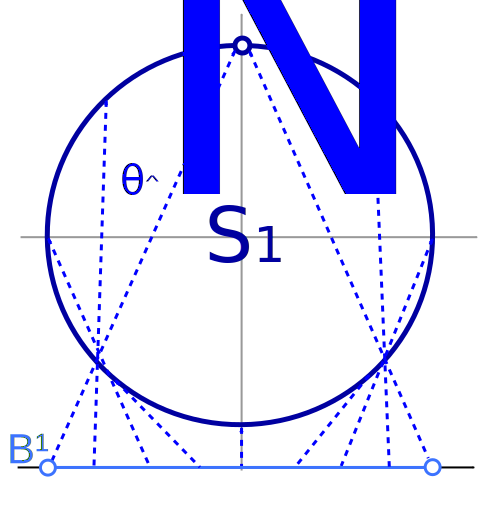
\includegraphics[width=\textwidth]{Bilder/keine-ueberdeckung.pdf}
                 \caption{\Cref{bsp:ohneNS}}
         \end{subfigure}%
 			\qquad\qquad
         \begin{subfigure}[b]{0.3\textwidth}
                 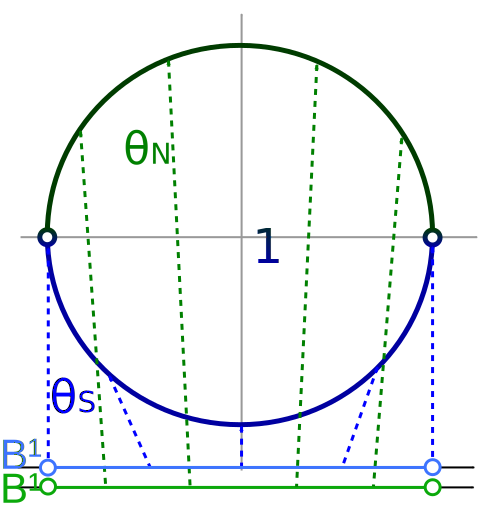
\includegraphics[width=\textwidth]{Bilder/ohne-aequator.pdf}
                 \caption{\Cref{bsp:keine-Ueberdeckung}}
         \end{subfigure}
         \caption{Kartenabbildungen für $S^1$}
\end{figure}

Ein weiteres Problem ist, dass aus der Surjektivität von $\Theta$ zwar die Injektivität von $K$ folgt, nicht aber umgekehrt:

\begin{bsp}\label{bsp:keine-Ueberdeckung}Die Karten 
	\[\theta_S: B^1 \to S^1: r \mapsto \exp{0,5 \pi i (r-1)} \text{ und } \theta_N: B^1 \to S^1: r \mapsto \exp{0,5 \pi i (1-r)}\]
bilden keine vollständige Überdeckung von $S^1$ (die beiden Äquatorpunkte werden nicht getroffen). Dennoch wäre $K$ zu diesen Karten bereits injektiv. Denn gilt für zwei Abbildungen $\tau, \psi \in \stetig(S^1)$, dass $(\tau\circ\theta_S, \tau\circ\theta_N) = K(\tau) = K(\psi) = (\psi\circ\theta_S, \psi\circ\theta_N)$ ist, so können sich $\tau$ und $\psi$ höchstens noch an den Äquatorpunkten unterscheiden. Da $\tau$ und $\psi$ aber stetig sind, sind diese beiden Punkte bereits durch ihre Umgebung eindeutig festgelegt. Folglich müssen $\tau$ und $\psi$ auch hier übereinstimmen und sind damit identisch.
\end{bsp}

Insgesamt sehen wir also, dass die Surjektivität der Algebrenkarten eine zu starke Forderung ist, während die Injektivität von $K$ anscheinend eine zu schwache Bedingung ist. 

\subsection{Satz und Beweis}

Der Versuch die in den Vorüberlegungen aufgetauchten Probleme zu beseitigen, führt uns zu der folgenden Charakterisierung von \CAlgMann.

\begin{defn}[kompakte Konvergenz]\label{defn:komKonv}
Sei ein topologischer Raum $X$ und eine Folge von Funktionen $(\psi_l: X \to \CC)_{l \in \NN}$ gegeben. Diese Folge \emph{konvergiert kompakt} gegen eine Funktion $\psi: X \to \CC$, wenn die Folge auf jeder kompakten Teilmenge von $X$ gleichmäßig gegen $\psi$ konvergiert.
\end{defn}

\begin{defn}[\CAlgMann]\label{defn:CAM}
Eine \CAlg{} $\A$ heißt \emph{\CAlgMan{} der Dimension $m$}, wenn es stetige Algebrenhomomorphismen
	\[k_i: \A \to \stetig^b(B^m), ~i = 1, \dots , N\]
gibt (für ein $N \in N$), sodass gilt:
\begin{defenum}
	\item \label{defn:CAM:surj}
	Zu allen $i \leq N$ und $\psi \in \stetig(\overline{B^m})$ mit $\psi|_{\partial B^m} \equiv \mathrm{const.}$ gibt es ein $a \in \A$, sodass $k_i(a) = \psi|_{B^n}$.
	\item \label{defn:CAM:kompkonv}
	Sind $(a_l)_{l \in \mathbb{N}} \subset \A$ und $\psi_i \in \stetig(B^m)$ mit
	\[\forall i: k_i(a_l) \overset{l \to \infty}{\longrightarrow} \psi_i \text{ konvergiert kompakt,}\]
	dann $\exists a \in \A: a_l \overset{l \to \infty}{\longrightarrow} a$ (Konvergenz in $\A$).
\end{defenum}
Diese Abbildungen bezeichnen wir als \emph{Algebrenkarten}.
\end{defn}

\begin{bem}
\ref{defn:CAM:surj} ist eine Art abgeschwächte Surjektivität: Es muss nämlich nur eine bestimmte Teilmenge der stetigen Abbildungen auf $\overline{B^m}$ getroffen werden. Die Einschränkung auf Abbildungen, die auf dem Rand konstant sind, verhindert gerade das Problem aus \Cref{bsp:ohneNS}.

Entsprechend unterbindet \ref{defn:CAM:kompkonv} das Problem aus \Cref{bsp:keine-Ueberdeckung} (wähle dazu eine Folge von Abbildungen in $\stetig(S^1)$, die gegen eine Abbildung konvergiert, die gerade an den beiden Äquatorpunkten Polstellen besitzt). Diese Eigenschaft ist dabei eine stärkere Forderung als die bloße Injektivität von $K$, d.h. die Injektivität dieser Abbildung folgt aus \ref*{defn:CAM:kompkonv}: Sind nämlich $a,b \in \A$, sodass für alle $i \leq N$ gilt $k_i(a) = k_i(b)$, dann ist $(k_i(a), k_i(b), k_i(a), k_i(b), \dots)$ eine konstante Folge und damit (kompakt) konvergent. Nach \ref*{defn:CAM:kompkonv} konvergiert dann auch $(a, b, a, b, \dots)$ in $\A$ und somit muss $a = b$ gelten.
\end{bem}

\begin{bem}
Die Dimension $m$ einer \CAlgMan{} $\A$ ist nicht identisch zu der Dimension $n$, die $\A$ als Vektorraum bzw. \CAlg{} besitzt. Allerdings werden wir sehen, dass sowieso immer nur einer der beiden Dimensionsbegriffe von Interesse ist. 

Ist nämlich die Dimension einer \CAlgMan{} $\A$ größer als $0$, so auch die der zugehörigen topologischen Mannigfaltigkeit $\SpecC(\A)$ (siehe den Beweis zu \Cref{satz:GD2}). Dann kann $\SpecC(\A)$ aber keine endliche Menge sein und daher $\A$ nach \Cref{sec:Anwendung} als \CAlg{} nicht mehr endlich dimensional. Ist umgekehrt die Dimension von $\A$ als \CAlg{} endlich, so muss die Dimension von $\A$ als \CAlgMan{} bereits $0$ sein.
\end{bem}

\begin{satz}[Gelfand-Dualität für \komenTopMan]\label{satz:GD2}
Die Kategorie der kompakten topologischen Mannigfaltigkeiten $\KatTopMan$ ist dual zu der der \CAlgMann{} $\KatCAlgMan$.
\end{satz}

\begin{proof}Wir verwenden hier die gleichen Funktoren wie in der gewöhnlichen Gelfand-Dualität (\Cref{satz:GD}):
	\[\begin{array}{@{}rrcl@{}}
	 			&\KatTopMan			&\simeq		&\KatCAlgMan^\op 												\\
	\stetig: 	&X					&\mapsto	&\stetig(X)													\\
				&(\varphi:X \to Y)	&\mapsto	&(h_\varphi: \stetig(Y) \to \stetig(X): \tau \mapsto \tau \circ \varphi)^\op 		\\
	\SpecC:		&\SpecC(\A)													&\mapsfrom	&\A				\\
				&(\varphi_h: \SpecC(\A) \to \SpecC(\B): f \mapsto f \circ h)	&\mapsfrom	&(h: \B \to \A)^\op
	\end{array}\]
Nun ist jede \komTopMan{} auch ein kompakter Hausdorffraum und zwei \komenTopMan{} sind isomorph genau dann, wenn sie es als kompakte Hausdorffräume sind (da beide Kategorien die gleichen Morphismen besitzen). Analog ist jede \CAlgMan{} auch eine \CAlg{} und zwei \CAlgMann{} sind isomorph genau dann, wenn sie es als \CAlgn{} sind. Die Dualität der Kategorien folgt also im Wesentlichen schon aus der gewöhnlichen Gelfand-Dualität (\Cref{satz:GD}).

Zu zeigen ist allerdings noch, dass die Funktoren in obiger Form überhaupt wohldefiniert sind, das heißt, dass $\stetig$ jeder \komenTopMan{} eine \CAlgMan{} zuordnet und umgekehrt $\SpecC$ jeder \CAlgMan{} eine \komTopMan{}.

Sei dazu zunächst $X$ eine \komTopMan{}. Dann gibt es nach \Cref{prop:topManAlt} Karten $\theta_i: B^m \to X$, sodass $(\theta_i(\overline{B_{0,5}^m}))_{i=1,\dots,N}$ eine Überdeckung von $X$ bilden. Daraus  definieren wir uns wie folgt Algebrenkarten:
	\[k_i: \stetig(X) \to \stetig^b(B^m): \tau \mapsto \tau \circ \theta_i \]
Zu zeigen ist nun also:
\begin{proofenum}
	\item \label{proof:GD2:kAlghom}
		Die $k_i$ sind stetige Algebrenhomomorphismen.
	\item \label{proof:GD2:schwachsurj}
		Zu allen $i \leq N$ und $\psi \in \stetig(\overline{B^m})$ mit $\psi|_{\partial B^m} \equiv \mathrm{const.}$ gibt es ein $\tau \in \stetig(B^m)$, sodass $k_i(\tau) = \psi|_{B^m}$.
	\item \label{proof:GD2:komkonv}
		Sind $(\tau_l)_{l \in \NN} \subset \stetig(X)$ und $\psi_i \in \stetig(B^m)$ so, dass
			\[\forall i: k_i(\tau_l) \overset{l \to \infty}{\longrightarrow} \psi_i \text{ kompakt konvergiert,}\]
		dann $\exists \tau \in \stetig(X): \tau_l \overset{l \to \infty}{\longrightarrow} \tau$.
	\setcounter{temp}{\value{proofenumi}}
\end{proofenum}

Zu \ref{proof:GD2:kAlghom}: Dass $k_i$ ein Algebrenhomomorphismus ist, zeigt sich durch einfaches Nachrechnen der entsprechenden Axiome. Für die Stetigkeit sei $\tau \in \stetig(X), ~\epsilon > 0$, dann gilt für alle $\psi \in \stetig(X)$ mit $\norm{\tau - \psi} < \epsilon $:
\begin{align*}
\norm{k_i(\tau)-k_i(\psi)} &= \norm{\tau \circ \theta_i - \psi \circ \theta_i} = \underset{r \in B^m}{\sup} |\tau \circ \theta_i(r) - \psi \circ \theta_i(r)| \\
 &\leq \underset{x \in X}{\sup} |\tau (x) - \psi (x)| = \norm{\tau- \psi} < \epsilon
\end{align*}
Also ist $k_i$ ein stetiger Algebrenhomomorphismus.

Zu \ref{proof:GD2:schwachsurj}: Sei $\psi \in \stetig(\overline{B^m} )$ mit $\psi|_{\partial B^m} \equiv \lambda \in \mathbb{C}$ und $i \leq N$. Dann definiere:
\[\tau: X \to \CC: x \mapsto \begin{cases} \psi(\theta_i^{-1}(x)) &, x \in \theta_i(B^m) \\ \lambda &, \text{ sonst} \end{cases} \]
Diese Abbildung hat die gewünschte Eigenschaft:
\[k_i(\tau) = \tau \circ \theta_i = \psi \circ \theta_i^{-1} \circ \theta_i = \psi|_{B^m}\]
Noch zu zeigen ist, dass $\tau$ auch tatsächlich stetig ist. Dazu sei $x \in X$ und $\epsilon > 0$ beliebig.
\Fall{1} $x \in \theta_i(B^m)$ bzw. $\theta^{-1}(x) \in B^m$

Da $\psi$ stetig ist, existiert ein $\delta > 0$, sodass gilt: 
	\[\forall r \in B^m: \norm{r - \theta_i^{-1}(x)} <\delta \Rightarrow \left|\psi(r) - \psi(\theta_i^{-1}(x))\right| < \epsilon \]
Dann ist $\theta_i\left(B_\delta^m(\theta_i^{-1}(x)) \cap B^m\right) \subseteq X$ eine offene Umgebung von $x$ und es gilt für alle $y \in \theta_i\left(B_\delta^m(\theta_i^{-1}(x)) \cap B^m\right)$, dass $\theta_i^{-1}(y) \in B_\delta^m(\theta_i^{-1}(x))$, also
	\[\left|\tau(y) - \tau(x)\right| = \left|\psi(\theta_i^{-1}(y)) - \psi(\theta_i^{-1}(x))\right| < \epsilon.\]

\Fall{2} $x \notin \theta_i(B^m)$, d.h. $\tau(x) = \lambda$.

Da $\psi \in \stetig(\overline{B^m})$ ist, gibt es insbesondere für alle $r \in \partial B^m$ ein $\delta_r > 0 $, sodass
	\[\forall s \in B_{\delta_r}^m(r) \cap \overline{B^m}: |\psi(s) - \lambda| = |\psi(s) - \psi(r)| < \epsilon.\]
Nun ist $U := \bigcup_{r \in \partial B^m}B_{\delta_r}^m(r) \supseteq \partial B^m$ offen und daher $\overline{B^m} \backslash U$ und $\theta_i\left(\overline{B^m} \backslash U\right)$ abgeschlossen. Folglich ist $X \backslash \theta_i\left(\overline{B^m} \backslash U\right) \supset X \backslash \theta_i(\overline{B^m})$ eine offene Umgebung von $x$ und es gilt:
	\[\forall y \in X \backslash \theta_i\left(\overline{B^m} \backslash U\right): \left|\psi(y) - \psi(x)\right| = \begin{cases} |\psi(\theta_i^{-1}(y)) - \lambda| < \epsilon &, y \in U \cap \overline{B^m} \\ |\lambda - \lambda| = 0 < \epsilon &, \text{ sonst}\end{cases}\]
In beiden Fällen ist $\tau$ also stetig.

Zu \ref{proof:GD2:komkonv}: Seien $ (\tau_l)_{l\in \mathbb{N}} \subset \stetig(X), ~\psi_i \in \stetig(B^m)$ so, dass
\[\forall i: k_i(\tau_l) \overset{l \to \infty}{\longrightarrow} \psi_i ~\text{kompakt konvergiert.}\]
Dann definiere:
\[\tau: X \to \mathbb{C}: x \mapsto \psi_i(r), \text{ mit } r\in B^m \text{ und } i\in \{1,\dots,N\} \text{ so, dass } \theta_i(r) = x \]
Dies ist wohldefiniert, denn
\begin{itemize}
  \item $(\theta_i(B^m))_{i\in\{1,\dots,N\}}$ ist Überdeckung von $X$, also können $i$ und $r$ wie verlangt gewählt werden.
  \item Seien $i,j \in \{1,\dots,N\}$ und $r,s \in B^m$ so, dass $\theta_i(r) = x = \theta_j(s)$. Dann gilt (da $\{r\}, \{s\} \subset B^m$ kompakt):
  \[\psi_i(r) = \underset{l \to \infty}{\lim} \tau_l\circ\theta_i(r) = \underset{l \to \infty}{\lim} \tau_l (x) = \underset{l \to \infty}{\lim} \tau_l\circ\theta_j(s) = \psi_j(s)\]
\end{itemize}

Ferner ist $\tau$ stetig, denn für jedes $x \in X$ gibt es eine offene Umgebung $B_\epsilon^m(\theta_i^{-1}(x)) \subseteq B^m$ von $\theta_i^{-1}(x)$ und damit eine offene Umgebung $\theta_i(B_\epsilon^m(\theta_i^{-1}(x)))$ von $x$. Auf dieser ist $\tau$ identisch zu $\psi \circ \theta_i^{-1}$, welches eine stetige Abbildung ist. Also ist $\tau$ stetig in $x$ und entsprechend auf ganz $X$.

Noch zu zeigen ist, dass die $\tau_l$ gleichmäßig gegen $\tau$ konvergieren. Da für jedes $i \leq N$ die $k_i(\tau_l)$ kompakt gegen $\psi_i$ konvergieren, konvergieren diese auf der kompakten Menge $\overline{B_{0,5}^m}$ gleichmäßig. Das heißt für jedes $\epsilon > 0$ gibt es ein $L_i \in \NN$, sodass
	\[\forall l \geq L_i, r \in \overline{B_{0,5}^m}: \left| k_i(\tau_l)(r) - \psi_i(r) \right| < \epsilon.\]
Also gilt für $L := \max\{L_1, \dots, L_N\}$ und alle $i \leq N$:
	\[\forall l \geq L, r \in \overline{B_{0,5}^m}: \left|\tau_l(\theta_i(r)) - \tau(\theta_i(r))\right| = \left|k_i(\tau_l)(r) - \psi(r)\right|  < \epsilon\]
Aus $\bigcup_{i=1}^N\theta_i(\overline{B_{0,5}^m}) = X$ folgt damit, dass die $\tau_l$ auf ganz $X$ gleichmäßig gegen $\tau$ konvergieren. Also ist $\tau \in \stetig(X)$ und $\tau_l \overset{l \to \infty}{\longrightarrow} \tau$.

Insgesamt folgt aus \ref{proof:GD2:kAlghom}, \ref{proof:GD2:schwachsurj} und \ref{proof:GD2:komkonv}, dass die $k_i$ tatsächlich Algebrenkarten sind und $\stetig(X)$ somit eine \CAlgMan{} ist.


Bleibt noch die andere Richtung: Sei dazu $\A$ eine \CAlgMan{}. Dann gibt es Algebrenkarten $k_i: \A \to \stetig^b(B^m)$. Daraus  definieren wir uns nun Karten für $\SpecC(\A)$:
	\[\theta_i: B^m \to \SpecC(\A): r \mapsto (f_r^i: \A \to \CC: a \mapsto k_i(a)(r)) \]
Zu zeigen ist jetzt:
\begin{proofenum}
	\setcounter{proofenumi}{\value{temp}}
	\item \label{proof:GD2:fAlghom}
		Die $f_r^i$ sind stetige Algebrenhomomorphismen.
	\item \label{proof:GD2:Homoeo}
		Die $\theta_i$ sind Homöomorphismen auf ihr Bild.
	\item \label{proof:GD2:Ueberdeckung}
		$(\theta_i(B^m))_{i\in\{1,\dots,N\}}$ ist eine Überdeckung von $\SpecC(\A)$.
\end{proofenum}
Dann ist $\SpecC(\A)$ nach \Cref{prop:topManAlt} eine \komTopMan.

Zu \ref{proof:GD2:fAlghom}: Dass $f_r^i$ ein Algebrenhomomorphismus ist, ergibt sich wieder durch Nachrechnen der Axiome. Zum Beweis der Stetigkeit sei $a \in \A$ und $\epsilon > 0$. Dann gibt es, da $k_i$ stetig, ein $\delta>0$ sodass 
\[\forall b \in \A: \norm{a-b} < \delta \Rightarrow \norm{k_i(a)-k_i(b)} < \epsilon\]
Damit gilt $\forall b \in \A$ mit $\norm{a-b} < \delta$
\[ |f_r^i(a) - f_r^i(b)| = |k_i(a)(r)-k_i(b)(r)| \leq \underset{s \in B^m}{\sup} |k_i(a)(s)-k_i(b)(s)| = \norm{k_i(a)-k_i(b)} < \epsilon\]
Also ist $f_r^i$ ein stetiger Algebrenhomomorphismus.

Zu \ref{proof:GD2:Homoeo}: \begin{itemize}
	\item $\theta_i$ ist injektiv, denn:
	
	Seien $r, s \in B^m$ mit $\theta_i(r) = \theta_i(s)$, d.h. 
	\begin{align*}
		\forall a \in \A: k_i(a)(r) = f_r^i(a) = \theta_i(r)(a) = \theta_i(s)(a) = f_s^i(a)  = k_i(a)(s)
	\end{align*}
	Angenommen es wäre $r \neq s$. Dann gäbe es nach dem Lemma von Urysohn ein stetiges $\psi: \overline{B^m} \to \mathbb{C}$ mit
	\[\psi|_{\partial B^m \cup \{r\}} \equiv 0, ~\psi(s) = 1\]
	Da $\A$ eine \CAlgMan{} ist, gibt es ein $a \in \A: k_i(a) = \psi|_{B^m}$. Also gilt 
	\[\theta_i(r)(a) = k_i(a)(r) = \psi(r) = 0 \neq 1 = \psi(s) = k_i(a)(s) = \theta_i(s)(a),\]
	was im Widerspruch zur Voraussetzung $\theta_i(r) = \theta_i(s)$ steht. Daher ist doch $r = s$.
	
	\item $\theta_i$ ist stetig, denn:
	
	Seien $r \in B^m, \epsilon > 0$ und $a \in \A$, also
	\[U_i(f_r^i, a, \epsilon) := \{f_s^i \in \theta_i(B^m) ~\big|~ |f_r^i(a) - f_s^i(a)| < \epsilon\}\]
	eine offene Umgebung von $f_r^i$. Dann ist $k_i(a) \in \stetig^b(B^m)$, d.h. 
	\[\exists \delta >0: \forall s \in B^m: |r-s| <\delta \Rightarrow |k_i(a)(r) - k_i(a)(s)| < \epsilon\]
	Damit gilt für alle $s \in B^m$ mit $|r-s| < \delta$:
	\[ |f_r^i(a) - f_s^i(a)| = |k_i(a)(r) - k_i(a)(s)| < \epsilon \]
	also $\theta_i(s) = f_s^i \in U_i(f_r^i, a, \epsilon)$.
	
	\item $(\theta_i|_{\theta_i(B^m)})^{-1}$ ist stetig, denn:
	
	Sei $f_r^i \in \theta_i(B^m), \epsilon>0$ (oBdA sei $\epsilon$ so klein, dass $B_\epsilon^m(r) \subset B^m$). Dann gibt es nach dem Lemma von Urysohn eine stetige Funktion
	\[\psi: \overline{B^m} \to \mathbb{C} \text{ mit } \psi|_{\overline{B^m}\backslash B_\epsilon^m(r)} \equiv 0, ~\psi(r) = 1\]
	Da $\A$ eine \CAlgMan{} ist, gibt es ein $a \in \A$ mit $k_i(a) = \psi|_{B^m}$.
	
	Damit gilt für alle $f_s^i \in U_i(f_r^i, a, 1)$:
	\[|1 - \psi(s)| = |\psi(r) - \psi(s)| = |\theta_i(a)(r) - \theta_i(a)(s)| = |f_r^i(a) - f_s^i(a)| < 1\]
	Also $\psi(s) \neq 0$ und damit nach Definition von $\psi$:
	\[s \notin \overline{B^m}\backslash B_\epsilon(r) \Rightarrow s \in B_\epsilon^m(r) \Rightarrow |r-s| < \epsilon\]
\end{itemize}
Damit ist $\theta_i$ ein Homöomorphismus auf ihr Bild.

Zu \ref{proof:GD2:Ueberdeckung}: \Ann $\exists f \in \SpecC(\A) \backslash \bigcup_{i=1}^N \theta_i(B^m)$.

Dann definiere 
\[W_l := \bigcup_{i=1}^N \theta_i(\overline{B_{1-\frac{1}{l}}(0)}) \subset \bigcup_{i=1}^N \theta_i(B^m)\]
Die $W_l$ sind als endliche Vereinigung abgeschlossener Mengen ebenfalls abgeschlossen. Damit existieren dem Lemma von Urysohn zu Folge ($\SpecC(\A)$ ist ein kompakter Hausdorffraum) stetige Funktionen
\[\psi_l: \SpecC(\A) \to \mathbb{C} \text{ mit } \psi_l|_{W_l} \equiv 0, ~\psi_l(f) = l.\]
Nun sind die $\psi_l \in \stetig(\SpecC(\A))$, welcher laut Satz von Gelfand-Neumark (\Cref{satz:GN}) isometrisch isomorph zu $\A$ ist. Nach Definition des Isomorphismuses $\AlgIso: \A \to  \stetig(\SpecC(\A))$ gibt es damit $a_l \in \A$, sodass:
\[\psi_l = \AlgIso(a_l) = \tau_{a_l}: f \mapsto f(a_l)\]
Ferner gilt für $r \in \overline{B_{1-\frac{1}{l}}^m(0)}$:
\[k_i(a_l)(r) = f_r^i(a_l) = \tau_{a_l}(f_r^i) = \psi_l(f_r^i) = \psi_l(\theta_i(r)) = 0\]
Sei $W \subset B^m$ kompakt, dann gibt es ein $L \in \mathbb{N}$, sodass $W \subset \overline{B_{1-\frac{1}{L}}^m(0)}$ und damit:
\[\forall l \geq L: W \subset \overline{B_{1-\frac{1}{l}}^m(0)} \text{, d.h. } k_i(a_l)|_W \equiv 0\]
Also konvergiert $k_i(a_l)$ kompakt gegen die Nullfunktion auf $\stetig(B^m)$ und es gibt ein $a \in \A$ mit $a_l \overset{l \to \infty}{\longrightarrow} a$. Folglich muss es auch ein $\psi \in \stetig(\SpecC(\A))$ geben, sodass $\psi_l \overset{l \to \infty}{\longrightarrow} \psi$. Für dieses gilt dann:
\[|l - \psi(f)| = |\psi_l(f) - \psi(f)| \leq \underset{g \in \SpecC(\A)}{\sup}|\psi_l(g) - h(g)| \overset{l \to \infty}{\longrightarrow} 0 \]
Also $|l - \psi(f)| \overset{l \to \infty}{\longrightarrow} 0$ und damit $\psi(f) = \infty ~\lightning$

Daher muss die Annahme falsch sein und doch $\SpecC(\A) = \bigcup_{i=1}^N \theta_i(B^m)$ gelten, d.h. $(\theta_i(B^m))_{i=1,\dots,N}$ eine Überdeckung von $\SpecC(\A)$ sein.

Aus \ref{proof:GD2:fAlghom}, \ref{proof:GD2:Homoeo} und \ref{proof:GD2:Ueberdeckung} folgt jetzt, dass $\SpecC(\A)$ eine topologische Mannigfaltigkeit ist. Damit ist die Wohldefiniertheit der Funktoren $\stetig$ und $\SpecC$ für \Cref{satz:GD2} gezeigt.
\end{proof}

Diese Erweiterung der Gelfand-Dualität für \komTopMann{} bestätigt nun, dass wir mit den in \Cref{defn:CAM} definierten \CAlgMann{} tatsächlich eine Klassifikation der zu $\KatTopMan$ dualen Kategorie $\KatCAlgMan$ gefunden haben. Können wir also für eine \CAlg{} zeigen, dass sie zusätzlich die Eigenschaften einer \CAlgMan{} besitzt (d.h. es entsprechende Algebrenkarten gibt), dann wissen wir bereits, dass der ihr durch die Gelfand-Dualität zugeordnete kompakte Hausdorffraum eine topologische Mannigfaltigkeit ist.
\newpage
\phantomsection
\addcontentsline{toc}{section}{Ausblick}
\section*{Ausblick}
\begin{center}
Sind nun alle Fragen beantwortet?
\end{center}

Nun, hoffentlich zumindest die in der Einleitung aufgeworfenen. Wir haben gesehen, dass \CAlgn{} als Räume stetiger komplexwertiger Funktionen über kompakten Hausdorffräumen aufgefasst werden können, haben gezeigt, dass die Kategorie der \CAlgn{} dual zu der der kompakten Hausdorffräume ist, und haben schließlich die zur Kategorie der \komTopMann{} duale Unterkategorie der \CAlgn{} gefunden. Aber wie so oft in der Mathematik bringt jede Antwort auch wieder neue Fragen mit sich.

So könnte man sich nun fragen, ob sich die \CAlgMann{} noch irgendwie \glqq schöner\grqq{} charakterisieren lassen. Etwa durch eine zusätzliche innere Struktur analog zur Involution, die die Struktur ist, deren Existenz die \CAlgn{} innerhalb der Banachalgebren charakterisiert. Auch wäre es interessant zu untersuchen, ob \CAlgMann{} irgendwelche besonderen Eigenschaften haben, die allgemeine \CAlgn{} nicht notwendigerweise besitzen.

Eine andere Frage könnte sein, was passiert, wenn wir eine andere Unterkategorie von $\KatTop$ bzw. $\KatTopMan$ betrachten - etwa die der (kompakten) differenzierbaren Mannigfaltigkeiten. Jede solche ist auch eine topologische Mannigfaltikeit, hat also eine duale \CAlgMan{}. Aber kann man einer \CAlgMan{} irgendwie ansehen, dass sie dual zu einer differenzierbaren Mannigfaltigkeit ist? Und lässt sich hierfür wiederum eine passende Erweiterung der Gelfand-Dualität finden? 

Gerade die letzte Frage dürfte vermutlich etwas aufwändiger zu beantworten sein als der Schritt von kompakten Hausdorffräumen zu topologischen Mannigfaltigkeiten. Denn im Gegensatz zu topologoischen Mannigfaltigkeiten sind zwei differenzierbare Mannigfaltigkeiten nicht automatisch \glqq gleich\grqq{} (diffeomorph), wenn sie es nur als topologische Räume sind\footnote{Ein berühmtes Beispiel hierfür sind die exotischen $S^7$ - siehe \cite{Elwes2011} für eine kurze Einführung und \cite{Bognat2011} für einen ausführlichen Beweis}. Hier müsste also erst eine zusätzliche Struktur auf \CAlgn{} definiert werden, anhand der sich auch eigentlich isomorphe \CAlgn{} in solchen Fällen unterscheiden lassen (also wenn sie zu homöomorphen, aber nicht diffeomorphen Mannigfaltigkeit \glqq gehören\grqq). Die Frage ist also:

\begin{center}
Was ist der Unterschied zwischen $\stetig(S^7)$ und $\stetig(S^7)$?
\end{center}

\newpage
\appendix

\section{Anhang}
\subsection{Sätze ohne Beweis}
Die folgenden Sätze wurden in dieser Arbeit ohne Beweis benutzt:

\begin{satz}[Satz von Banach-Alaoglu]\label{satz:BA}
Sei $(\A, \norm{.})$ ein normierter Vektorraum und $\dual{\A}$ der zugehörige Dualraum. Dann ist die abgeschlossene Einheitskugel
 \[\dual{B_1}(0) := \{f \in \dual{\A} ~|~ \norm{f} := \underset{\norm{a} = 1}{\sup}|f(a)| \leq 1\} \subset \dual{\A}\]
kompakt bezüglich der schwach-*-Topologie.
\end{satz}

Ein Beweis dieses Satzes findet sich bspw. bei \cite[Theorem VIII.3.11 \& Korollar VIII.3.12]{Werner2011}.


\begin{satz}[Lemma von Zorn]\label{satz:LZ}
Sei $(M, \leq)$ eine partiell geordnete Menge (d.h. eine nicht-leere Menge $M$ mit einer reflexiven, transitiven und anti-symetrischen Ordnung $\leq$), sodass jede total geordnete Teilmenge $N$ (d.h. für je zwei Elemente $n, \tilde{n} \in N$ gilt $\tilde{n} \leq n \vee n \leq \tilde{n}$) eine obere Schranke besitzt (d.h. ein $m \in M$ sodass für alle $n \in N$ gilt: $n \leq m$).

Dann gibt es in M ein maximales Element (d.h. ein $m \in M$ sodass es kein $\tilde{m} \in M$ mit $m < \tilde{m}$ gibt).
\end{satz}

Das Lemma von Zorn ist äquivalent zum Auswahlaxiom. Ein Beweis seiner Aussage findet sich in \cite[S. 214f]{Jaenich2008}.

\begin{satz}\label{satz:Quotient}
Ist $\A$ ein vollständiger normierter Vektorraum und $W \subseteq \A$ ein abgeschlossener Unterraum. Dann ist 
	\[^\A/_W := \{[a] ~|~ a \in \A \text{ mit } [a] = [b] \Leftrightarrow a-b \in W\}\]
mit
	\[[a] + [b] := [a+b],\qquad \lambda[a] := [\lambda a],\qquad \norm{[a]} := \inf_{x \in W}\norm{a+x}\]
ein vollständiger normierter Vektorraum.
\end{satz}

Ein Beweis zu diesem Satz findet sich in \cite[Satz I.3.2]{Werner2011}.

\begin{satz}[Satz von Stone-Weierstraß]\label{satz:SW}
Sei $X$ ein kompakter Hausdorffraum, $\stetig(X) :=\{\tau: X \to \CC ~|~ \tau \text{ stetig}\}$ der Raum der komplexwertigen, stetigen Funktionen auf $X$ und $\A \subseteq \stetig(X)$ eine Algebra mit folgenden Eigenschaften:
\begin{itemize}
	\item $\A$ enthält die konstanten Funktionen $X \to \CC: x \mapsto \lambda$.
	\item $\A$ trennt Punkte in $X$, d.h. für je zwei $x, y \in X$ mit $x \neq y$ gibt es eine Funktion $\tau \in \A$, sodass $\tau(x) \neq \tau(y)$.
	\item $\A$ ist selbstadjungiert, d.h. für alle $\tau \in \A$ ist auch $(\overline{\tau}: x \mapsto \overline{\tau(x)}) \in \A$.
\end{itemize}
Dann liegt $\A$ bezüglich der von der Supremumsnorm induzierten Topologie dicht in $\stetig(X)$.
\end{satz}

Ein Beweis dieses Satzes findet sich bspw. in \cite[Satz VIII.4.7]{Werner2011}.


\begin{satz}[Lemma von Urysohn]\label{satz:Ury}
Sei $X$ ein topologischer Raum, in dem je zwei disjunkte abgeschlossene Mengen immer disjunkte offene Umgebungen haben. Seien außerdem $V, W \subset X$ zwei disjunkte abgeschlossene Teilmengen. 

Dann gibt es eine stetige Funktion $\psi: X \to [0,1]$ mit $\psi|_V \equiv 0$ und $\psi|_W \equiv 1$.
\end{satz}

Ein Beweis dieses Aussage findet sich in \cite[S. 136-139]{Jaenich2008}. Ein Beispiel für topologische Räume, die die Voraussetzung des Lemmas von Urysohn erfüllen, sind kompakte Hausdorffräume (siehe \cite[S. 135 (Bemerkung)]{Jaenich2008}).





\newpage
\subsection{Diagramm zum Satz von Gelfand-Neumark}\label{sec:DiagramGN}
Dieses Diagramm veranschaulicht die verschiedenen Zwischenschritte im Beweis zum Satz von Gelfand-Neumark (\Cref{satz:GN}):

\begin{sideways}
	\begin{minipage}{18cm}
		\fontsize{8pt}{1.5}\selectfont
		{\crefname{prop}{Prop.}{Prop.}
\crefname{section}{Absch.}{Absch.}
\crefname{kor}{Kor.}{Kor.}
\tikzstyle{Def} = [rectangle, draw, fill=gray!50, 
    text width=4.5em, text badly centered]
\tikzstyle{Prop} = [rectangle, draw, 
    text centered, rounded corners]
\tikzstyle{Absch} = [rectangle, draw, 
    text centered]
\tikzstyle{keinBeweis} = [rectangle, fill=gray!35, 
    text centered]    
\tikzstyle{Text} = [ 
    text centered]
\tikzstyle{BewTeil} = []

\tikzstyle{line} = [draw, -latex']
\tikzstyle{line2} = [draw]

\begin{tikzpicture}[node distance = 6em, auto]

\node [Text] (satz) {\large $\AlgIso: \A \to \stetig(\SpecC(\A)): a \mapsto \left(\tau_a:f \mapsto f(a)\right)$};
	\node [BewTeil, left of=satz, node distance=40em] (legende) {\large Legende:};
		\node [keinBeweis, below of=legende, node distance=2em, text width=1em, text height=1em] (grau) {};
		\node [BewTeil, right of=grau, node distance=10em, text width=17em] (grau-erk) {= ohne Beweis verwendete Aussage};
		\node [Absch, below of=grau, node distance=2em, text width=1em, text height=1em] (viereck) {};
		\node [BewTeil, right of=viereck, node distance=10em, text width=17em] (viereck-erk) {= wesentlicher Beweisschritt};
		\node [Prop, below of=viereck, node distance=2em, text width=1em, text height=1em] (rund) {};
		\node [BewTeil, right of=rund, node distance=10em, text width=17em] (rund-erk) {= Hilfsaussage};
	\node [below of=satz, node distance=3em] (hilf-satz) {};
    
    %Bijektiv-Block
    \node [Absch, left of=hilf-satz, node distance=16em, text width=8em] (bi) {\cref{sec:Bijektiv} \\ $\AlgIso$ bijektiv};    
    	\node [below of=bi](hilf-bi) {}; 
    	\node [Text, left of=hilf-bi, node distance=8em] (inj) {$\AlgIso$ injektiv};
    			\node [left of=inj, node distance=18em] (links-inj) {};
       		%Isomometrisch
    		\node [Absch, below of=inj, text width=8em] (iso) {\cref{sec:isometrisch} \\ $\AlgIso$ isometrisch};
				\node [below of=iso](hilf-iso) {};     
    			\node [Prop, left of=hilf-iso, node distance=13em, text width=8em] (RAnorm) 
    			{\cref{prop:R-gleich-Norm} \\ $R_\A(a) = \norm{a}$};
    					\node [below of=RAnorm, node distance=3em, text width=4em] (unter-RAnorm) {};
    				\node [Text, below of=RAnorm] (hilf-RAnorm) {};    				
    				\node [Prop, below of=hilf-RAnorm, text width=8em] (RAlima) 
    				{\cref{prop:R-groesser-lima} \\ in Banachalg.: \\ $R\!_\A(a)\!\!\geq\!\!\lim\!\norm{\!a^k\!}^\frac{1}{k}$}; 
    				\node [Prop, below of=RAlima, text width=8em] (konv)
    				{\cref{prop:Konvergenz} \\ $\alpha_n \to \epsilon < 1$ \\ $\Rightarrow (\alpha_n)^n \to 0$};
       			\node [Prop, right of=hilf-iso, node distance=10em, text width=15em] (fasigma) 
       			{\cref{prop:Spektrum-von-a} \\ $\{f(a)|f\in\SpecC(\A)\}=\sigma_\A(a)$};
					\node [BewTeil, below of=fasigma] (bew-fasigma) 
					{\qquad für $\lambda \in \sigma_\A(a)$:};
					\node [BewTeil, below of=bew-fasigma, text width=10em, node distance=1.5em] (bew-fasigma1) 
					{\ref{proof:Spektrum-von-a:maxIdeal} $(\lambda e-a)\A \subseteq I_\lambda$ \\ \qquad\!\!\!\!\! max. Ideal};
						\node [keinBeweis, left of=bew-fasigma1, node distance=12em] (zorn) 
						{Lemma v. Zorn (\ref{satz:LZ})};						
					\node [BewTeil, below of=bew-fasigma1, text width=10em, node distance=2.5em] (bew-fasigma2) 
					{\ref{proof:Spektrum-von-a:I-abg} $I_\lambda$ abg.};										    		
							\node [left of=bew-fasigma2, node distance=6.5em] (links-bew-fasigma2) {};
					\node [BewTeil, below of=bew-fasigma2, text width=10em, node distance=2em] (bew-fasigma3) 
					{\ref{proof:Spektrum-von-a:AI-BA} $^\A/_{I_\lambda}$ BA \& Körper};	
						\node [keinBeweis, left of=bew-fasigma3, node distance=12em] (quotient) 
						{Quatientenalg. (\ref{satz:Quotient})};						
					\node [BewTeil, below of=bew-fasigma3, text width=10em, node distance=2em] (bew-fasigma4) 
					{\ref{proof:Spektrum-von-a:Projektion} $f:\A \to {}^\A/_{I_\lambda} \cong \CC$};
						\node [Prop, left of=bew-fasigma4, node distance=12em] (nichtleer) 
						{\cref{kor:spektrum-nicht-leer}: $\sigma_\A(a) \neq \emptyset$};						
				    
    	\node [Text, right of=hilf-bi, node distance=8em] (sur) {$\AlgIso$ surjektiv};
			\node [below of=sur](hilf-sur) {};     
    		\node [Text, left of=hilf-sur, node distance=5em] (HAabg) {$\AlgIso(\A)$ abg.};
    		\node [Text, right of=hilf-sur, node distance=5em] (HAdicht) {$\AlgIso(\A)$ dicht};
				\node [below of=HAdicht] (hilf-HAdicht) {};
					\node [keinBeweis, right of=hilf-HAdicht, text width=7em, node distance=4.3em] (SW) 
					{Satz v. Stone-Weiherstraß (\ref{satz:SW})};   
				\node [BewTeil, below of=hilf-HAdicht] (bew-HAdicht) {$\SpecC(\A) \dots$};
				\node [BewTeil, below of=bew-HAdicht, text width=8.4em, node distance=2em] (bew-HAdicht1) 
				{$\bullet$ ist kompakt};
						\node [right of=bew-HAdicht1, node distance=7em] (rechts-bew-HAdicht1) {};	
				\node [BewTeil, below of=bew-HAdicht1, text width=8.4em, node distance=2em] (bew-HAdicht2) 
				{$\bullet$ enth. konst. Fkt.};
						\node [right of=bew-HAdicht2, node distance=5em] (rechts-bew-HAdicht2) {};
				\node [BewTeil, below of=bew-HAdicht2, text width=8.4em, node distance=2em] (bew-HAdicht3) 
				{$\bullet$ trennt Pkte.};	
				\node [BewTeil, below of=bew-HAdicht3, text width=8.4em, node distance=2em] (bew-HAdicht4) 
				{$\bullet$ ist selbstadj.};	

	% Sternhom-Block
    \node [Absch, right of=hilf-satz, node distance=11em, text width=10em] (sternhom) 
    {\cref{sec:CAlgHom} \\ $\AlgIso$ \CAlgHom}; 
    		\node [right of=sternhom] (rechts-sternhom) {}; 
    	\node [Text, below of=sternhom] (stern) {$\AlgIso(a^*) = (\AlgIso(a))^*$};    
    			\node [left of=stern, node distance=5.5em] (links-stern) {}; 
      	\node [Prop, below of=stern, text width=8em] (sternkonj) 
    	{\cref{prop:Stern-zu-Konjugation} \\ für $f: \A \to \CC$ \\ Alghom.: \\ $f(a^*) = \overline{f(a)}$};
    	\node [Prop, below of=sternkonj, text width=8em] (selbstadj) 
    	{\cref{prop:Spektrum-reell} \\ für $a$ selbstadj.: \\ $\sigma_\A(a) \subseteq \RR$};
    			\node [below of=selbstadj, node distance=3em, text width=4em] (unter-selbstadj) {};    	
    	\node [Prop, below of=selbstadj, text width=8em] (eEig) 
    	{\cref{lemma:CAlg-Eigenschaften} \\ $\norm{e} = 1$, $e^* = e$};
    	%Lemma 1.15 (Spec komp.)
    	\node [Absch, below of=eEig, text width=8em] (Speckomp) {\cref{lemma:MA} \\ $\SpecC(\A)$ komp. HD-Raum}; 
    	\node [keinBeweis, below of=Speckomp, text width=8em] (alaoglu) {Satz v. Banach-Alaoglu (\ref{satz:BA})};     	
    	
    %Alghom	
	\node [Absch, below of=bew-HAdicht4, text width=15em, node distance=6.6em] (Alghom) 
	{\cref{sec:Algebrenhomomorphismus} \\ $\AlgIso$ Algebrenhomomorphismus};    	

	%stetig
	\node [Absch, below of=nichtleer, text width=8em, node distance=4em] (stetig) 
	{\cref{lemma:BAlg-Eigenschaften} \\ $+$, $\cdot$, $^{-1}$ stetig}; 


%Pfade:
	%Zu bijektiv:
	\path [line] (inj) -- (bi);
		\path [line] (iso) -- (inj);
			\path [line] (RAnorm) -- (iso);
				\path [line] (RAlima) -- (RAnorm);
					\path [line] (konv) -- (RAlima);
			\path [line] (fasigma) -- (iso);
				\path [line] (bew-fasigma) -- (fasigma);
					\path [line] (zorn) -- (bew-fasigma1);
					\path [line] (quotient) -- (bew-fasigma3);
					\path [line] (nichtleer) -- (bew-fasigma4);
						\path [line] (RAlima.east) -- (nichtleer.west);
	\path [line] (sur) -- (bi);
		\path [line] (HAabg) -- (sur);
			\path [line] (iso) -- (HAabg);
		\path [line] (HAdicht) -- (sur);
			\path [line] (bew-HAdicht) -- (HAdicht);
				\path [line2] (Speckomp) -| (rechts-bew-HAdicht1.center);
					\path [line] (rechts-bew-HAdicht1.center) -- (bew-HAdicht1);
					\path [line] (alaoglu) -- (Speckomp);
	%Zu Sternhom:
	\path [line] (stern) -- (sternhom);
	\path [line] (sternkonj) -- (stern);
		\path [line] (fasigma) -- (sternkonj.west);
	\path [line] (selbstadj) -- (sternkonj);
	\path [line] (eEig) -- (selbstadj);	
	
    %Von Algebrenhomomorphismus:
    \path [line2] (Alghom.east) -| (rechts-sternhom.east);
        \path [line] (rechts-sternhom.east) -- (sternhom);
    \path [line2] (Alghom.north -| rechts-bew-HAdicht2.east) -- (rechts-bew-HAdicht2.east);
    	\path [line] (rechts-bew-HAdicht2.east) -- (bew-HAdicht2);
    \path [line2] (Alghom.west) -| (links-inj.west);
	    \path [line] (links-inj.west) -- (inj);
	\path [line2] (Alghom.north -| hilf-sur) -- (fasigma.south -| hilf-sur);
		\path [line] (fasigma.north -| hilf-sur) |- (HAabg);
	
	%Von stetig:
	\path [line] (stetig.west) -- (RAlima);
	\path [line2] (stetig.east) -| (links-bew-fasigma2.center);
		\path [line] (links-bew-fasigma2.center) -- (bew-fasigma2);
	    
	%Von stern zu selbstadj    
    \path [line2] (stern.west) -- (links-stern.east);
	    \path [line] (links-stern.east) |- (bew-HAdicht4);
	    
	%Von SW:
	\path [line2] (SW) -- (hilf-HAdicht.center);	
	
	%RAlima nach selbstadj
	\path [line2] (RAnorm.south -| unter-RAnorm.east) -- (unter-RAnorm.east);
		\path [line2] (unter-RAnorm) -- (unter-selbstadj);
		\path [line] (unter-selbstadj.west) -- (selbstadj.south -| unter-selbstadj.west);    
	          
\end{tikzpicture}
}
	\end{minipage}
\end{sideways}


\newpage
\nocite{*}
\printbibliography

\end{document}
